\documentclass{article}
\usepackage[english]{babel}
%\usepackage[utf8x]{inputenc}
%\usepackage{apacite}
\usepackage[toc,page]{appendix}
%\usepackage{biblatex} % place in the document preamble
%%---------- path ------------%%
%\def\input@path{{~/Dropbox/6_Graduate/}}
%%---------- my command --- ----------%%
\newcommand{\pard[1]}{\frac{\partial}{\partial{#1}}}
\newcommand{\mean[1]}{\frac{1}{n}\sum_{i=1}^{#1}}
\newcommand{\defeq}{\vcentcolon=}
\newcommand{\eqdef}{=\vcentcolon}
\newcommand\independent{\protect\mathpalette{\protect\independenT}{\perp}}
\newcommand{\wh}{\widehat}
\newcommand{\itl}{\intercal}
\newcommand{\p}{\prime}
\newcommand{\bs}{ \boldsymbol}
\newcommand{\mb}{\mathbb}
\newcommand{\ml}{\mathcal}
\newcommand{\br}{\bar}
\newcommand{\txt}{\text}
\newcommand{\lt}{\left}
\newcommand{\rt}{\right}
\newcommand{\lv}{\lvert}
\newcommand{\rv}{\rvert}
\newcommand{\nlim}{\underset{n \to \infty}{\lim}}
\newcommand{\smb}{\begin{bmatrix}}
	\newcommand{\sme}{\end{bmatrix}}
\newcommand\indep{\protect\mathpalette{\protect\independenT}{\perp}}
\def\independenT#1#2{\mathrel{\rlap{$#1#2$}\mkern2mu{#1#2}}}
\newcommand{\tsgn}{\txt{sgn}}


%%-------- my package -------%%
\usepackage{ragged2e}
\usepackage{float}
\usepackage{epstopdf}
\usepackage[final]{pdfpages}
%\usepackage{cite}
\usepackage{amsmath}
\usepackage{color}
\usepackage{graphicx}
\usepackage{verbatim}
\usepackage{commath}
\usepackage{caption}
%\usepackage{bbm}
%\usepackage{xfrac}
%\usepackage{dsfont}
\usepackage{amssymb}
\usepackage{verbatim}
\usepackage{mathtools}
\usepackage{resizegather}
\usepackage{xfrac}
\usepackage{amsthm}
\usepackage[ruled]{algorithm2e}
%\newtheorem{remark}{Remark}
%\newtheorem{lemma}{Lemma}
%\newtheorem{theorem}{Theorem}
%\newtheorem{corollary}{Corollary}
\newtheorem{theorem}{Theorem}[section]
\newtheorem{lemma}[theorem]{Lemma}
\newtheorem{proposition}[theorem]{Proposition}
\newtheorem{corollary}[theorem]{Corollary}
\renewcommand\qedsymbol{$\blacksquare$}

%%----------------------------------------------------------------------------%%
%%------------------------------ Import Packages -----------------------------%%
%%----------------------------------------------------------------------------%%


\usepackage{booktabs}  % professionally typeset tables
\usepackage{amsmath}
\usepackage{textcomp}  % better copyright sign, among other things
\usepackage{xcolor}
\usepackage{lipsum}    % filler text
\usepackage{subfig}    % composite figures


%%----------------------------------------------------------------------------%%
%%---------------------------- Formatting Options ----------------------------%%
%%----------------------------------------------------------------------------%%
%%

%% -------------------------------------------------------------------------- %%
%% Disposition format -- any titles, headings, section titles
%%  These formatting commands affect all headings, titles, headings,
%%  so sizing commands should not be used here.
%%  Formatting options to consider are
%%     +  \sffamily - sans serif fonts.  Dispositions are often typeset in
%%                    sans serif, so this is a good option. 
%%     +  \rmfamily - serif fonts
%%     +  \bfseries - bold face
%\dispositionformat{\sffamily\bfseries}   % bold and sans serif


%% ------------------------------
\title{Multiple-stage Dynamic Treatment Regimes under Constraints}
\author{Shuping Ruan, Eric Laber\\ Department of Statistics, North Carolina State University}


\begin{document}
\maketitle

\section{Introduction}
Dynamic treatment regimes (DTRs), also known as adaptive treatment strategies or policies, are sequences of decision rules of which input is time-varying patient information and output is a recommended treatment at each intervention point~\cite{Chakraborty2014, Moodie2004, Murphy2003}. These decision rules can be used to inform treatment decision for chronic conditions, e.g., depression, alcohol and drug abuse, HIV infection, cancer, diabetes etc., where clinicians have to make decisions at each stage based on evolving patient histories. A handful of methods have been developed to estimate the optimal treatment regimes. For example, indirect methods include Q-learning~\cite{Nahum2012}, penalized Q-learning~\cite{Song2011}, interactive Q-learning~\cite{Linn2014}, A-learning~\cite{Schulte2014}, regret-regression~\cite{henderson2010}, g-estimation~\cite{gestimation} and so on. Policy search methods include marginal structural mean models~\cite{Robins2000,Orellana2010a}, outcome weighted learning~\cite{Zhao2012,Zhang2012,Zhao2015}, doubly robust estimators~\cite{Zhang2012b}, and so forth. However, these methods only take a single clinical outcome into consideration, and neglect the clinical need to balance several competing outcomes. For example, a clinician may have to balance treatment effectiveness, side-effect burden, and cost while developing a treatment strategy for a patient with a chronic disease; or maximize the expected time to an adverse event while controlling the variance of the time to the adverse event.\\

Although handling the trade-off among multiple competing outcomes is important in practice, there has been little work done on this issue.  Lizotte et al. proposed to compute the optimal treatment regimes of all the possible linear combinations of two competing outcomes~\cite{Lizotte2010}. However, only considering linear trade-off between two competing outcomes may not be sufficient to describe all possible patient preferences~\cite{LaberTwo2014}. Wang et al. considered a compound score or ``expert score" by numerically combining information on treatment efficacy, toxicity, and the risk of disease progression~\cite{Wang2012}. Unfortunately, it can be difficult to elicit a good composite outcome, and the quality of the estimated treatment regime maybe severely affect by the misspecification of a composite outcome~\cite{Laber2014}. Some methods do not require the formation of composite outcomes. For example, set-valued dynamic treatment regimes proposed by Laber et al. inputs current patient information and outputs a set of recommended treatments. Multiple treatments may included in the set recommended, unless there exists a treatment that is best across all outcomes. Domain expertise is needed for tie breaking when a set of several treatments are recommended. Also, it needs to specify ``clinically significant differences" for competing outcomes~\cite{LaberTwo2014}. \\

In this chapter, we continue the work previously done by Linn at el.~\cite{constrained}, and propose a new statistical framework to tackle the problem of balancing multiple competing outcomes using constrained estimation. By restricting the values of secondary ones, we search for the feasible regimes with the maximized value of the primary outcome, ie., constrained optimal regimes. This method is useful, for example, when the clinicians need to find an adaptive intervention strategy that maximize the effectiveness and controls the side-effect burden simultaneously. This chapter focuses on constrained optimal regimes under the multiple stage setting. Data are assumed to be from Sequential, Multiple Assignment, Randomized Trials~\cite{Lei2012}. Observational data can also fit in our framework if the additional assumptions about the treatment assignment mechanism are tenable. However, precaution is needed when using data from observational studies, as one key assumption, the no unmeasured confounder assumption, can not be verified~\cite{Chakraborty2013}. 

\section{Methodology}
\subsection{Define multi-stage constrained optimal treatment regimes }
\subsubsection{Dataset}
 The dataset is denoted by $$\{(\bs{X}_{1}^{i}, A_{1}^{i},\bs{X}_{2}^{i}, A_{2}^{i}, \cdots, \bs{X}_{T}^{i}, A_{T}^{i}, \bs{Y}^{i})\}_{i=1}^{n},$$ which is composed of $n$ identically, independently distributed patient trajectories\\ $\{(\bs{X}_{1}, A_{1},\bs{X}_{2}, A_{2}, \cdots, \bs{X}_{T}, A_{T}, \bs{Y})\}$. Capital letters denote random variables; lower case letters denote realized values of these random variables. Let $\bs{X}_1$ be a patient baseline covariate, $A_1$ be the first-stage treatment variable, $\bs{X}_2$ be the patient covariate collected between first decision point and second decision point, $A_2$ be the second-stage treatment variable. So on, and so forth. Finally, $\bs{X}_T$ is the patient intermediate outcomes collected at the final decision point $T$, $A_T$ is the treatment assignment at that time point, and $\bs{Y}$ is the final outcome vector. For $t = 1, \cdots, T$, $\bs{X}_t\in \bs{\ml{X}}_t \subseteq{\mb{R}^{p_t}}$, $A_{t} \in \ml{A}_t = \{ 1, 2, \cdots, m_t\}$, and $\bs{Y} \in \mb{R}^J$. The first component $Y_1$ denote the primary outcome of interest, which is coded so that larger values are more desirable. Meanwhile, $Y_2, \cdots, Y_J$ are the secondary outcomes of interest, which are coded so that lower is better. Let $\bs{H}_t$ denote the patient history information up to the decision point $t$, i.e., $\bs{H}^\itl_1 = (1, \bs{X}^\itl_1)$, $\bs{H}^\itl_2 = ( \bs{H}^\itl_1, A_1, \bs{X}^\itl_2)$, $\cdots$,  $\bs{H}^\itl_t = (\bs{H}^\itl_{t-1}, A_{t-1}, \bs{X}^\itl_t)$, $\cdots$, $\bs{H}^\itl_T = (\bs{H}^\itl_{T-1}, A_{T-1}, \bs{X}^\itl_T)$. Besides, let $\br{A}_t = (A_1, A_2, \cdots, A_t)$ denotes a sequence of treatment history up to time point $t$, and $\br{A}_t \in \br{\ml{A}_t}$, where $\br{\ml{A}_t} = \ml{A}_1 \times \ml{A}_2 \times \cdots \times \ml{A}_t$, $t =2 , \cdots, T$. %Note $\br{A}_1 = A_1$ and $\br{\ml{A}}_1 = \ml{A}_1$. %Besides, let $\bs{W}= (\bs{X}_{2},  \, A_{2}, \, \cdots,\, \bs{X}_{T},  \, A_{T}, \bs{Y})$. 
 
 \subsubsection{Potential outcomes}
 The potential outcome or counter-factual framework by Neyman, Rubin and Robins are adopted to identify the causal effect of a regime. The set of potential outcomes is $\bs{W}^* = \{ \bs{X}^*_2(a_1), \bs{X}^*_3(\br{a}_2), \cdots, \bs{X}^*_T(\br{a}_{T-1}), \bs{Y}^*_T(\br{a}_T), \text{for all } \br{a}_t \in \br{\ml{A}}_t, t=1, 2, \cdots, T \}$, where $\bs{X}^*_t(\br{a}_{t-1})$ is the potential outcome that would have been observed if the patient followed the treatment history sequence $\br{a}_{t-1}$. The following three necessary assumptions are necessary to connect  observed data with potential outcomes~\cite{Neyman, Rubin2005, Rubin1980, Robins1997, Hernan2006}.
 \begin{itemize}
 	\item \textit{B1. Consistency:}
 	 $\bs{Y} = \bs{Y}^*(\br{A}_T)$, and $\bs{X}_t = \bs{X}^*_t(\br{A}_{t-1})$, $t = 2, \cdots, T$.
 	\item \textit{B2. Sequential randomization assumption:}
 	$A_{t}  \indep \bs{W}^*  \mid \bs{H}_{t}$ for $t =1 ,2, \cdots, T$.
 	\item \textit{B3. Positivity assumption:} $\exists \, \epsilon_t > 0$, such that $\text{Pr}(A_t = a_t \mid \bs{H}_t=\bs{h}_t) > \epsilon_t$, for all $a_t \in \ml{A}_t$, $t=1, 2, \cdots, T$.
 \end{itemize}
B1) states that the intermediate and final outcomes observed equal to the patient's intermediate and final potential outcomes under the sequence of treatment actually assigned. It also implies no interference among individuals. B2) mean that conditional on the observed patient history $\bs{H}_t$, the treatment at time point $t$ is assigned independently of the his or her potential outcomes. B3) guarantees a positive possibility for any $a_t \in \ml{A}_t$ having been assigned to patients with $\bs{H}_t = \bs{h}_t$. These assumptions imply that $\txt{Pr}(\bs{Y}^*(\br{a}_T) \le \bs{y} \,| \, \bs{H}^*_T(\br{a}_{T-1}) =\bs{h}_T) = \txt{Pr}(\bs{Y} \le \bs{y} \, |\,  \bs{H}_T = \bs{h}_T, A_T=a_T)$ and $\txt{Pr}(\bs{X}_{t+1}^*(\br{a}_{t}) \le \bs{x}_{t+1} \,|\, \bs{H}^*_t(\br{a}_{t-1}) = \bs{h}^*_t) = \txt{Pr}(\bs{X}_{t+1} \le \bs{x}_{t+1} \mid  \bs{H}_t = \bs{h}_t, A_t=a_t)$ for $t = 1, 2, \cdots, T-1$. Hence, we can estimate the values of a regime using the observed dataset.
\subsubsection{Define constrained optimal dynamic treatment regimes }
A dynamic treatment regime, $\bs{\pi} = (\pi_1, \pi_2, \cdots, \pi_T)$, is a sequence of decision rules. Each decision rule, $\pi_t : \text{supp}( \bs{H}_t ) \to \ml{A}_t$, is a function that maps the support of patient history information $\bs{H}_t$ to the set of all possible treatments at time point $t$. The final potential outcome under the regime $\bs{\pi}$ is $\bs{Y}^*(\bs{\pi}) = \sum_{\br{a}_T \in \br{\ml{A}}_T}\bs{Y}^*(\br{a}_T)\mb{I}(\bs{\pi} = \br{a}_T)$, and the intermediate potential outcome under that regime is $\bs{X}_{t+1}^*(\bs{\pi}_{t}) = \sum_{\br{a}_t \in \br{\ml{A}}_t}\bs{X}_{t+1}^*(\br{a}_{t})\mb{I}(\bs{\pi}_t = \br{a}_t)$, where $\bs{\pi}_t = (\pi_1, \pi_2, \cdots, \pi_t)$. The value of a dynamic treatment regime, $\bs{V}(\bs{\pi}) = \mb{E}\bs{Y}^*(\bs{\pi})$, is defined as the expected final outcome if each patient in the population of interest is treated according to $\bs{\pi}$. Each component of $\bs{V}(\bs{\pi})$ is denoted by $V_j(\bs{\pi}) = \mb{E}Y_j^*(\bs{\pi})$, for $j = 1, \cdots, J$. Our goal is to find a constrained optimal regime, $\bs{\pi}_{\bs{\nu}}^{*}$, that maximizes the expectation of the primary final potential outcome $V_1\left( \bs{\pi}\right) $, subject to an upper bound constraints on the expectation of the secondary final potential outcomes $V_j\left( \bs{\pi}\right)$, for $j=2 ,\cdots, J$.  The $J-1$ dimensional vector of upper bounds is denoted as $\bs{\nu} = (\nu_1, \nu_2, \cdots, \nu_{J-1})$, which can be determined by the preference of clinicians or patients.  Therefore, a multi-stage constrained optimal regime problem is defined as
\begin{equation}
\begin{gathered}
 \underset{\bs{\pi} \in \bs{\Pi}}{\txt{max}} \,\,
 V_1( \bs{\pi} )  \\
  \txt{subject to}  \,\, V_j( \bs{\pi} ) \le \nu_{j-1},
\end{gathered}
\end{equation}
where $j = 2, 3, \cdots, J$  and $\bs{\Pi}$ is the class of dynamic treatment regimes under consideration. The feasible space of the class of regimes, $\ml{F}(\bs{\Pi})$, is the set of all regimes satisfying the constraints. For each $\bs{\pi} \in \ml{F}(\bs{\Pi})$, $V_j(\bs{\pi}) \le \nu_{j-1}$, for $j = 2, \cdots, J$. Then, a multi-stage constrained optimal regime can also be written as $\bs{\pi}_{\bs{\nu}}^*= \text{argmax}_{{\bs{\pi} \in \ml{F}(\bs{\Pi})}}V_1 (\bs{\pi})$.\\

We choose the class of regime to be the class of linear decision rules, where each mapping function $\pi_t$ at time point $t$ is indexed by $\bs{\theta}_t$. More specifically, $\pi_t(\bs{h}_t) = \tsgn(\bs{h}^{\itl}_t\bs{\theta}_t)$. Hence, all $V_j(\bs{\pi})$'s can be considered as functions of $\bs{\theta}$ and can be exchangeably denoted $V_j(\bs{\theta})$'s. As only the directions of $\bs{h}^\itl_t\bs{\theta}_t$ matters, we restrict $\bs{\theta}_t$ to be unit vectors, i.e., $\bs{\theta}^\itl_t\bs{\theta}_t = 1$, for $t = 1, \cdots, T$. Then, problem (2.1) above can be written as
\begin{equation}
\begin{gathered}
\max_{\bs{\theta} \in \bs{\Theta}} V_1(\bs{\theta})\\
\,\, \txt{subject to}\,
V_j(\bs{\theta}) - \nu_j \le 0,\\
\hspace{2.0cm} \bs{\theta}_t^\itl \bs{\theta}_t^\itl - 1 =0.
\end{gathered}
 \end{equation}
where $\bs{\theta} = (\bs{\theta}_1, \cdots, \bs{\theta}_T)$, $j =2, \cdots, J$ and $t = 1, \cdots, T$. Let the feasible set of $\bs{\Theta}$ be $\ml{F}(\bs{\Theta})$, such that $V_j(\bs{\theta}) \le \nu_j$,  for any $\bs{\theta} \in \ml{F}(\bs{\Theta})$ and $j = 2, \cdots, J$. Then, the corresponding index parameter of a constrained optimal dynamic treatment regime is $\bs{\theta}^*_{\bs{\nu}} =\text{argmax}_{\bs{\theta} \in \ml{F}(\bs{\Theta})}V_1(\bs{\theta})$, and $\bs{\theta}^*_{\bs{\nu}} = (\bs{\theta}^*_{\bs{\nu},1}, \bs{\theta}^*_{\bs{\nu},2}, \cdots, \bs{\theta}^*_{\bs{\nu},T})$.

\begin{comment}
\textbf{ Convergence of the Penalty-Barrier Trajectory  $\bs{\theta}^*_{\kappa}(\mu)$  to $\bs{\tau}^0_{\kappa}$}\\

\textbf{ Convergence in probabilty of the estimator  to $\hat{\bs{\tau}}_{\kappa}(\mu)$ to  the Penalty-Barrier Trajectory  $\bs{\tau}^*_{\kappa}(\mu)$} \\

%\mnote{ convergence $\hat{\tau}_{\kappa}(\mu) \overset{p}{\to} \tau^*_{\kappa}(\mu) \to  \tau^0_{\kappa}(\mu)$}

Step 1:  $\underset{\bs{\tau}, \| \bs{\tau}_1 \|^2 = 1, \| \bs{\tau}_2 \|^2 = 1}{\sup} \mid \hat{S} (\bs{\tau}, \mu) -S^*( \bs{\tau}, \mu)  \mid = o_p(1)$ \\

Let $S^*(\bs{\tau}, \mu) = \mb{E} Y^*(\bs{\tau}) + \mu \txt{log} \lt\{ \kappa - \mb{E} Z^*(\bs{\tau}) \rt\} - \frac{1}{2\mu} \lt\{ (\bs{\tau}_1^\itl \bs{\tau}_1 -1 )^2 + (\bs{\tau}_2^\itl \bs{\tau}_2 -1 )^2 \rt\},$ and $\widehat{S}(\bs{\tau}, \mu) = \wh{\mb{E}} Y(\bs{\tau}) + \mu \, \txt{log} \lt\{ \kappa - \wh{\mb{E}}Z(\bs{\tau}) \rt\} - \frac{1}{2\mu} \lt\{ (\bs{\tau}_1^\itl \bs{\tau}_1 -1 )^2 + (\bs{\tau}_2^\itl \bs{\tau}_2 -1 )^2 \rt\},$ then
$$\widehat{S}(\bs{\tau}, \mu) - S^*(\bs{\tau}, \mu) = \hat{\mb{E}} Y(\bs{\tau}) - \mb{E} Y^*(\bs{\tau})  + \mu \, \txt{log}\frac{ \kappa - \hat{\mb{E}}Z(\bs{\tau})}{ \kappa - \mb{E} Z^*(\bs{\tau})}$$

First look at $\hat{\mb{E}} Y_n(\bs{\tau}) - \mb{E} Y^*(\bs{\tau})$

$Y_n(\bs{\tau}) \sim F_{Y_n}(y;\bs{\tau})$

If $Y_n(\bs{\tau}) \overset{d}{\to} Y^*(\bs{\tau})$, aka, $\wh{F}_{Y_n}(y;\bs{\tau}) \to F_Y(y;\bs{\tau}), \text{as } n \to \infty$, for all $y$ at which $F_Y(\cdot, \bs{\tau})$ is continuous. Also,  for each $\bs{\tau}$, if there exists some random variable $T$, such that  $|Y_n(\bs{\tau})| \le |T|$ for all $n$ and $\mb{E} |T| \le \infty$, then $\wh{\mb{E}} Y_n(\bs{\tau}) \to \mb{E} Y^*(\bs{\tau})$.
Thus, we have $\wh{\mb{E}} Y_n(\bs{\tau}) - \mb{E} Y^*(\bs{\tau}) = o_p(1)$ \\

Step 2:  conditions for $\wh{F}_{Y_n}(y;\bs{\tau}) \to F_Y(y;\bs{\tau}), \text{as } n \to \infty$\\

Step 3:  Consistency of $\wh{\bs{\tau}}_{n,\kappa} \to \bs{\tau}^*_{\kappa}$. It can be proven by following similar proof in Lemma 2 at one-stage. \\

Step 4: Asymptotic Normality of $\wh{\bs{\tau}}_{n,\kappa}$ \\
Taylor expansion, for each $\mu$ \\

$\nabla\wh{S}(\bs{\tau}^*_{\bs{\nu}}(\mu)) = \nabla\wh{S}(\wh{\bs{\tau}}_{\bs{\nu}}(\mu)) - \nabla^2\wh{S}(\tilde{\bs{\tau}}_{\bs{\nu}}(\mu) ) (\wh{\bs{\tau}}_{\bs{\nu}}(\mu) - \bs{\tau}^*_{\bs{\nu}}(\mu) )$


$\sqrt{n}\nabla\wh{S}(\bs{\tau}^*_{\bs{\nu}}(\mu)) =  -\sqrt{n} \nabla^2\wh{S}(\tilde{\bs{\tau}}_{\bs{\nu}}(\mu) ) (\wh{\bs{\tau}}_{\bs{\nu}}(\mu) - \bs{\tau}^*_{\bs{\nu}}(\mu) )$

\begin{flalign*}
\nabla\wh{S}(\bs{\tau}^*_{\bs{\nu}}(\mu)) = \nabla \mb{E} Y(\bs{\tau}) - \mu \frac{\nabla \mb{E} Z(\bs{\tau})}{  \kappa - \mb{E} Z(\bs{\tau}) }
\end{flalign*}

\begin{flalign*}
\nabla^2\wh{S}(\bs{\tau}^*_{\bs{\nu}}(\mu)) = \nabla^2 \mb{E} Y(\bs{\tau}) - \mu \frac{\nabla^2 \mb{E} Z(\bs{\tau}) \lt[ \kappa - \mb{E} Z(\bs{\tau}) \rt] + \{ \nabla \mb{E} Z(\bs{\tau}) \}^2}{  \lt\{\kappa - \mb{E} Z(\bs{\tau}) \rt\}^2}
\end{flalign*}
\begin{flalign*}
& \nabla \wh{\mb{E}} Y(\bs{\tau})\\
= & \nabla\int y \,d \wh{F}_{Y(\bs{\tau})}(y) \\
= &  \nabla\int y \lt[ \,d \iint  F_{\epsilon}\lt\{ y - m_Y - \tsgn(r_2)c_Y\rt\}\,d G_{Y}\lt\{ m_Y, c_Y, r_2 \mid \bs{h}_1 , d_1(\bs{h}_1)\rt\} \,d F_{\bs{H}_1}(\bs{h}_1) \rt] \\
= &  \nabla\int y \lt[ \,d \iint  F_{\epsilon}\lt\{ y - m_Y - \tsgn(r_2)c_Y\rt\}\,d G_{Y}\lt\{ m_Y, c_Y, r_2 \mid \bs{h}_1 , d_1(\bs{h}_1)\rt\} \,d F_{\bs{H}_1}(\bs{h}_1) \rt]
\end{flalign*}
Assuming $d G_Y$ is correctly specified and is differentiable and continuous
\\

Step 5: Projected CI for $\wh{\mb{E}} Y_n(\wh{\bs{\tau}}_{n,\kappa})$

Is $d F - d \hat{F} = d(F - \hat{F})$ ??\\
Note:
convergence $\hat{\tau}_{\kappa}(\mu) \overset{p}{\to} \tau^*_{\kappa}(\mu) \to  \tau^0_{\kappa}(\mu)$
\begin{flalign*}
&  \hat{\mb{E}} Y(\bs{\tau}) - \mb{E} Y^*(\bs{\tau})  \\
= & \int y \,d \wh{F}_{Y_d} (y) - \int y \,d F_{Y^*_d} (y) \\
= &  \int y  \lt\{  \,d\wh{F}_{Y_d} (y) - \,d F_{Y^*_d} (y) \rt\}  \\
% = & \int y  \lt\{ \wh{f}_{Y_d} (y) - f_{Y^*_d} (y) \rt\} \,dy
\end{flalign*}
If for any arbitrary $\bs{d}$, $d F_{Y^*_{\bs{d}}} (y) $ is a density and $d\wh{F}_{Y_{\bs{d}}}(y)$ is a uniformly consistent estimator; that is $\underset{y}{\sup} \mid d\wh{F}_{Y_d} (y) - d F_{Y^*_d} (y) \mid =o_p(1)$, then

\begin{flalign*}
&  \hat{\mb{E}} Y(\bs{\tau}) - \mb{E} Y^*(\bs{\tau})  \\
= & \int y \,d \wh{F}_{Y_d} (y) - \int y \,d F_{Y^*_d} (y) \\
= &  \int y  \lt\{  \,d\wh{F}_{Y_d} (y) - \,d F_{Y^*_d} (y) \rt\}  \\
\le & \int \mid y \mid \, dy  \cdot o_p(1) \\
% = & \int y  \lt\{ \wh{f}_{Y_d} (y) - f_{Y^*_d} (y) \rt\} \,dy\\
= &  \iint  F_{\varepsilon_Y}\lt[ y - m(\bs{h}_2) - \tsgn\lt\{r_2(\bs{h}_2; \bs{\tau}_2)\rt\}c_Y(\bs{h}_2) \rt] \,d G_{Y}\lt\{ m_Y, c_Y, r_2 \rvert \bs{h}_1 , d_1(\bs{h}_1)\rt\} \,d F_{\bs{H}_1}(\bs{h}_1)
\end{flalign*}

\newpage
\textbf{Reference}\\

\textbf{Convergence in Distribution}\\
Suppose that $(X_1, X_2, \dots)$ and $X$ are real-valued random variables with distribution functions $(F_1, F_2,  \dots)$ and $F$, respectively. We say that the distribution of $X_n$ converges to the distribution of $X$ as $n \to \infty$ if
$$F_n(x) \to F(x), \text{as } n \to \infty$$
for all $x$ at which $F$ is continuous. \\
% Link https://www.probabilitycourse.com/chapter7/7_2_4_convergence_in_distribution.php

\textbf{Lebesgue's Dominated Convergence Theorem}\\
If for some random variable $Z$, $| X_n | \le | Z |$ for all $n$ and $\mb{E} | Z | \le \infty$, then $X_n \overset{d}{\to} X$ implies that $\mb{E} X_n \to \mb{E} X$.

\end{comment}

\begin{comment}
\textbf{ Convergence of the Penalty-Barrier Trajectory  $\bs{\tau}^*_{\kappa}(\mu)$  to $\bs{\tau}^0_{\kappa}$}\\

\textbf{ Convergence in probabilty of the estimator  to $\hat{\bs{\tau}}_{\kappa}(\mu)$ to  the Penalty-Barrier Trajectory  $\bs{\tau}^*_{\kappa}(\mu)$} \\

%\mnote{ convergence $\hat{\tau}_{\kappa}(\mu) \overset{p}{\to} \tau^*_{\kappa}(\mu) \to  \tau^0_{\kappa}(\mu)$}

Step 1:  $\underset{\bs{\tau}, \| \bs{\tau}_1 \|^2 = 1, \| \bs{\tau}_2 \|^2 = 1}{\sup} \mid \hat{S} (\bs{\tau}, \mu) -S^*( \bs{\tau}, \mu)  \mid = o_p(1)$ \\

Let $S^*(\bs{\tau}, \mu) = \mb{E} Y^*(\bs{\tau}) + \mu \txt{log} \lt\{ \kappa - \mb{E} Z^*(\bs{\tau}) \rt\} - \frac{1}{2\mu} \lt\{ (\bs{\tau}_1^\itl \bs{\tau}_1 -1 )^2 + (\bs{\tau}_2^\itl \bs{\tau}_2 -1 )^2 \rt\},$ and $\widehat{S}(\bs{\tau}, \mu) = \wh{\mb{E}} Y(\bs{\tau}) + \mu \, \txt{log} \lt\{ \kappa - \wh{\mb{E}}Z(\bs{\tau}) \rt\} - \frac{1}{2\mu} \lt\{ (\bs{\tau}_1^\itl \bs{\tau}_1 -1 )^2 + (\bs{\tau}_2^\itl \bs{\tau}_2 -1 )^2 \rt\},$ then
$$\widehat{S}(\bs{\tau}, \mu) - S^*(\bs{\tau}, \mu) = \hat{\mb{E}} Y(\bs{\tau}) - \mb{E} Y^*(\bs{\tau})  + \mu \, \txt{log}\frac{ \kappa - \hat{\mb{E}}Z(\bs{\tau})}{ \kappa - \mb{E} Z^*(\bs{\tau})}$$

First look at $\hat{\mb{E}} Y_n(\bs{\tau}) - \mb{E} Y^*(\bs{\tau})$

$Y_n(\bs{\tau}) \sim F_{Y_n}(y;\bs{\tau})$

If $Y_n(\bs{\tau}) \overset{d}{\to} Y^*(\bs{\tau})$, aka, $\wh{F}_{Y_n}(y;\bs{\tau}) \to F_Y(y;\bs{\tau}), \text{as } n \to \infty$, for all $y$ at which $F_Y(\cdot, \bs{\tau})$ is continuous. Also,  for each $\bs{\tau}$, if there exists some random variable $T$, such that  $|Y_n(\bs{\tau})| \le |T|$ for all $n$ and $\mb{E} |T| \le \infty$, then $\wh{\mb{E}} Y_n(\bs{\tau}) \to \mb{E} Y^*(\bs{\tau})$.
Thus, we have $\wh{\mb{E}} Y_n(\bs{\tau}) - \mb{E} Y^*(\bs{\tau}) = o_p(1)$ \\

Step 2:  conditions for $\wh{F}_{Y_n}(y;\bs{\tau}) \to F_Y(y;\bs{\tau}), \text{as } n \to \infty$\\

Step 3:  Consistency of $\wh{\bs{\tau}}_{n,\kappa} \to \bs{\tau}^*_{\kappa}$. It can be proven by following similar proof in Lemma 2 at one-stage. \\

Step 4: Asymptotic Normality of $\wh{\bs{\tau}}_{n,\kappa}$ \\
Taylor expansion, for each $\mu$ \\

$\nabla\wh{S}(\bs{\tau}^*_{\bs{\nu}}(\mu)) = \nabla\wh{S}(\wh{\bs{\tau}}_{\bs{\nu}}(\mu)) - \nabla^2\wh{S}(\tilde{\bs{\tau}}_{\bs{\nu}}(\mu) ) (\wh{\bs{\tau}}_{\bs{\nu}}(\mu) - \bs{\tau}^*_{\bs{\nu}}(\mu) )$


$\sqrt{n}\nabla\wh{S}(\bs{\tau}^*_{\bs{\nu}}(\mu)) =  -\sqrt{n} \nabla^2\wh{S}(\tilde{\bs{\tau}}_{\bs{\nu}}(\mu) ) (\wh{\bs{\tau}}_{\kappa,\mu} - \bs{\tau}^*_{\kappa,\mu} )$

\begin{flalign*}
\nabla\wh{S}(\bs{\tau}^*_{\kappa,\mu}) = \nabla \mb{E} Y(\bs{\tau}) - \mu \frac{\nabla \mb{E} Z(\bs{\tau})}{  \kappa - \mb{E} Z(\bs{\tau}) }
\end{flalign*}

\begin{flalign*}
\nabla^2\wh{S}(\bs{\tau}^*_{\kappa,\mu}) = \nabla^2 \mb{E} Y(\bs{\tau}) - \mu \frac{\nabla^2 \mb{E} Z(\bs{\tau}) \lt[ \kappa - \mb{E} Z(\bs{\tau}) \rt] + \{ \nabla \mb{E} Z(\bs{\tau}) \}^2}{  \lt\{\kappa - \mb{E} Z(\bs{\tau}) \rt\}^2}
\end{flalign*}
\begin{flalign*}
& \nabla \wh{\mb{E}} Y(\bs{\tau})\\
= & \nabla\int y \,d \wh{F}_{Y(\bs{\tau})}(y) \\
= &  \nabla\int y \lt[ \,d \iint  F_{\epsilon}\lt\{ y - m_Y - \tsgn(r_2)c_Y\rt\}\,d G_{Y}\lt\{ m_Y, c_Y, r_2 \mid \bs{h}_1 , d_1(\bs{h}_1)\rt\} \,d F_{\bs{H}_1}(\bs{h}_1) \rt] \\
= &  \nabla\int y \lt[ \,d \iint  F_{\epsilon}\lt\{ y - m_Y - \tsgn(r_2)c_Y\rt\}\,d G_{Y}\lt\{ m_Y, c_Y, r_2 \mid \bs{h}_1 , d_1(\bs{h}_1)\rt\} \,d F_{\bs{H}_1}(\bs{h}_1) \rt]
\end{flalign*}
Assuming $d G_Y$ is correctly specified and is differentiable and continuous
\\

Step 5: Projected CI for $\wh{\mb{E}} Y_n(\wh{\bs{\tau}}_{n,\kappa})$

Is $d F - d \hat{F} = d(F - \hat{F})$ ??\\
Note:
convergence $\hat{\tau}_{\kappa}(\mu) \overset{p}{\to} \tau^*_{\kappa}(\mu) \to  \tau^0_{\kappa}(\mu)$
\begin{flalign*}
&  \hat{\mb{E}} Y(\bs{\tau}) - \mb{E} Y^*(\bs{\tau})  \\
= & \int y \,d \wh{F}_{Y_d} (y) - \int y \,d F_{Y^*_d} (y) \\
= &  \int y  \lt\{  \,d\wh{F}_{Y_d} (y) - \,d F_{Y^*_d} (y) \rt\}  \\
% = & \int y  \lt\{ \wh{f}_{Y_d} (y) - f_{Y^*_d} (y) \rt\} \,dy
\end{flalign*}
If for any arbitrary $\bs{d}$, $d F_{Y^*_{\bs{d}}} (y) $ is a density and $d\wh{F}_{Y_{\bs{d}}}(y)$ is a uniformly consistent estimator; that is $\underset{y}{\sup} \mid d\wh{F}_{Y_d} (y) - d F_{Y^*_d} (y) \mid =o_p(1)$, then

\begin{flalign*}
&  \hat{\mb{E}} Y(\bs{\tau}) - \mb{E} Y^*(\bs{\tau})  \\
= & \int y \,d \wh{F}_{Y_d} (y) - \int y \,d F_{Y^*_d} (y) \\
= &  \int y  \lt\{  \,d\wh{F}_{Y_d} (y) - \,d F_{Y^*_d} (y) \rt\}  \\
\le & \int \mid y \mid \, dy  \cdot o_p(1) \\
% = & \int y  \lt\{ \wh{f}_{Y_d} (y) - f_{Y^*_d} (y) \rt\} \,dy\\
= &  \iint  F_{\varepsilon_Y}\lt[ y - m(\bs{h}_2) - \tsgn\lt\{r_2(\bs{h}_2; \bs{\tau}_2)\rt\}c_Y(\bs{h}_2) \rt] \,d G_{Y}\lt\{ m_Y, c_Y, r_2 \rvert \bs{h}_1 , d_1(\bs{h}_1)\rt\} \,d F_{\bs{H}_1}(\bs{h}_1)
\end{flalign*}

\newpage
\textbf{Reference}\\

\textbf{Convergence in Distribution}\\
Suppose that $(X_1, X_2, \dots)$ and $X$ are real-valued random variables with distribution functions $(F_1, F_2,  \dots)$ and $F$, respectively. We say that the distribution of $X_n$ converges to the distribution of $X$ as $n \to \infty$ if
$$F_n(x) \to F(x), \text{as } n \to \infty$$
for all $x$ at which $F$ is continuous. \\
% Link https://www.probabilitycourse.com/chapter7/7_2_4_convergence_in_distribution.php

\textbf{Lebesgue's Dominated Convergence Theorem}\\
If for some random variable $Z$, $| X_n | \le | Z |$ for all $n$ and $\mb{E} | Z | \le \infty$, then $X_n \overset{d}{\to} X$ implies that $\mb{E} X_n \to \mb{E} X$.

\end{comment}

% modeling conditional distributions


\subsection{Re-define constrained optimal regimes via penalization}
Problem (2.2) is a nonlinear constrained continuous optimization task. It is solved via interior point method, where we re-formalize  the problem via quadratic-barrier penalization. To re-formalize the problem, we let $v_1(\bs{\theta}) = -V_1(\bs{\theta})$ and $v_j(\bs{\theta}) = V_j(\bs{\theta}) - \nu_j$ for $j = 2, \cdots, J$. Moreover, $h_t(\bs{\theta}_t) = \bs{\theta}_t^{\itl}\bs{\theta}_t - 1$. Hence, we have problem (2.2) equivalent to the following
\begin{equation}
\begin{gathered}
\min_{\bs{\theta} \in \bs{\Theta}} v_1(\bs{\theta})\\
\txt{subject to } v_j(\bs{\theta}) \le 0, \\
\hspace{2.0cm}h_t(\bs{\theta}_t) = 0.
\end{gathered}
\end{equation}
where $\bs{\theta} = (\bs{\theta}_1, \cdots, \bs{\theta}_T)$, $j =1, \cdots, J$ and $t = 1, \cdots, T$ . Interior point method approximate the solution of problem (2.3) by solving a sequence of the following problem (2.4), where $\mu$ is positive and approaches to zero in the limit. For each $\mu > 0$, the approximate problem is 
\begin{equation}
\min_{\bs{\theta}, \bs{z}} \phi_{\mu}(\bs{\theta}, \bs{z}) = \min v_1(\bs{\theta}) - \mu \sum_{j=2}^J \ln z_j, \text{subject to}\,\, v_j(\bs{\theta}) +z_j = 0, h_t(\bs{\theta}_t) = 0
\end{equation}
where $j=2, \cdots, J$ and $t = 1, \cdots, T$. $z_j$'s are the slack variables, which are restricted to be positive due the $\ln$ operator. The logarithmic terms, $\ln z_j$'s, are the barrier functions, which enforce the solution path to be within the feasible region of the problem (2.3). More details on interior points method can be found at section 2.1.2. \\

The sequence of solutions to problem (2.4) forms a trajectory path $\lt\{\bs{\theta}^*_{\nu}(\mu)\rt\}_{\mu\to0+}$ that convergence to the solution to problem (2.3) as $\mu \to 0$, i.e., $\lim_{\mu \to 0}\bs{\theta}^*_{\bs{\nu}}(\mu)=\bs{\theta}^*_{\bs{\nu}}$. The conditions for its convergence can be found at section 2.1.3. Let $\wh{\bs{V}}(\theta)$ be a consistent estimator of the values of a regime $\pi$. Then, correspondingly, $\wh{v}_1(\bs{\theta}) = -\wh{V}_1(\bs{\theta})$ and $\wh{v}_j(\bs{\theta})=\wh{\bs{V}}_j(\bs{\theta}) -\nu_j$ for $j = 2, \cdots, J$. Then, problem (2.4) with the plugin estimator is
\begin{equation}
\min_{\bs{\theta}, \bs{z}} \wh{\phi}_{\mu}(\bs{\theta}, \bs{z}) = \min \wh{v}_1(\bs{\theta}) - \mu \sum_{j=2}^J \ln z_j, \text{ subject to}\,\, \wh{v}_j(\bs{\theta}) +z_j = 0, h_t(\bs{\theta}_t) = 0,
\end{equation}
for $j=2, \cdots, J$ and $t=1, \cdots, T$. The solution to problem (2.5) is equivalent to the solution to penalty-barrier function below. 
\begin{equation}
\min_{\bs{\theta}} \wh{\phi}^{BP}_{\mu}(\bs{\theta}) = \min \wh{v}_1(\bs{\theta}) - \mu \sum_{j=2}^J \ln (-\wh{v}_j(\bs{\theta})) + \frac{1}{2\mu}\sum_{t=1}^{T}(\bs{\theta}^{\itl}_t\bs{\theta}_t - 1)^2
\end{equation}
Denote the solution to (2.5/2.6) as $\wh{\bs{\theta}}_{\nu}(\mu)$.We have proven that $\wh{\bs{\theta}}_{\nu}(\mu) \overset{p}{\to} \bs{\theta}^*_{\nu}(\mu)$. For the consistency of this estimator, the details and proof are provided in section 2.1.4 and appendix A.2.
\begin{comment}
\subsection{Convergence of penalty-barrier trajectory  $\bs{\theta}^*_{\bs{\nu}}(\mu)$}

We again examine the conditions under which the penalty-barrier trajectory $\bs{\tau}^*_{\kappa}(\mu)$ converges to the original constrained maximizer $\bs{\tau}^0_{\kappa}$, of which details are provided Appendix 1 Proof Draft 1. We specify  the conditions need(2.ed for our problem as follows. For notation simplicity in this section, we let $f(\bs{\tau}) = \mb{E} Y^*(\bs{\tau})$, $c_1 (\bs{\tau}) = \kappa - \mb{E}Z^*(\bs{\tau})$, $c_2(\bs{\tau}) = \bs{\tau}_1^\itl \bs{\tau}_1 - 1$, and $c_3(\bs{\tau}) = \bs{\tau}_2^\itl \bs{\tau}_2 - 1$. Let $g(\bs{\tau})$ denote the gradient of $f(\bs{\tau})$, i.e., $g(\bs{\tau}) = \nabla f(\bs{\tau}) = \nabla \mb{E}Y^*(\bs{\tau})$. Also, let $\bs{c}(\bs{\tau})$ be the vector of constraint functions $\{c_i(\bs{\tau})\}$, $i = 1, 2, 3$. The Jacobian matrix $\bs{c}^{\prime}(\bs{\tau})$ of first derivative of $\bs{c}(\bs{\tau})$ has row $\{\nabla c_{i}(\bs{\tau})\}^{\itl}$, and we use $J(\bs{\tau})$ to denote this Jacobian for concise.\\
 \begin{lemma}[Conditions for the trajectory $\{ \bs{\tau}_{\kappa}^*(\mu) \}$ converging to $\bs{\tau}^0_{\kappa}$\cite{Nocedal1999,fiacco,Forsgren2002}]
	Assume
	\begin{enumerate}
		\item the functions $f$, $c_1$, $c_2$, and $c_3$ are twice differentiable with respect to $\bs{\tau}$;
		\item the gradients $\nabla c_1$, $\nabla c_2$, and $\nabla c_3$ are linearly independent, where the gradients are taken with respect to $\bs{\tau}$;
		\item strict complementarity holds for  $\lambda_1^0 c_1(\bs{\tau}_{\kappa}^0) = 0$, where $\lambda_1^0$ is the Lagrangian multiplier of the inequality constraint $c_1$;
		\item the sufficient conditions under which $\bs{\tau}_{\kappa}^0$ be an isolated local constrained minimum of Problem (2) are satisfied by $(\bs{\tau}^0_{\kappa}, \bs{\lambda}^{0})$, where $\bs{\lambda}^0 = (\lambda_1^0, \lambda_2^0, \lambda_3^0)^\itl $ of which $\lambda_2^0$ is the  Lagrangian multipliers for the  constraint $c_2$, and $\lambda_3$ for $c_3$. The sufficient conditions for optimality are
		\begin{enumerate}
			\item $\bs{\tau}_{\kappa}^0$ is feasible and the LICQ (Linear Independence Constraint Qualification) holds at $\bs{\tau}_{\kappa}^0$, i.e., the Jacobian matrix of active constraints at $\bs{\tau}_{\kappa}^0$, $J_{\mathcal{A}}(\bs{\tau}_{\kappa}^0)$, has full row rank;
			\item $\bs{\tau}_{\kappa}^0$ is a KKT point and strict complementarity holds, i.e, the (necessarily unique) multiplier $\bs{\lambda}^0$ has the property that $\lambda_i^0 > 0$, for all $i  \in \mathcal{A}_{\mathcal{I}}(\bs{\tau}_{\kappa}^0)$, the set of indices of active inequality constraints at $\bs{\tau}_{\kappa}^0$;
			\item for all nonzero vectors $\bs{p}$ satisfying $J_{\mathcal{A}}(\bs{\tau}_{\kappa}^0)\bs{p} = 0$, there exists $\omega > 0$ such that $\bs{p}^{\intercal}H(\bs{\tau}_{\kappa}^0, \bs{\lambda}^0) \bs{p} \ge \omega \|\bs{p}\|^2$., where $H(\bs{\tau}_{\kappa}^0, \bs{\lambda}^0) $ is the hessian of the Lagrangian at $\bs{\tau}_{\kappa}^0$ and $\bs{\lambda}^0$, where $\bs{\lambda}^0$ is the vector of the Lagrangian multipliers, $\bs{\lambda}^0 = (\lambda_1^0, \lambda_2^0, \lambda_3^0)^{\intercal}$.
		\end{enumerate}
		then there is a positive neighborhood about $\mu = 0$ for which a unique-isolated differentiable function $\bs{\tau}^*_{\kappa}(\mu)$ exists. It describes a unique isolated trajectory of local maxima of $S^*(\bs{\tau}, \mu)$, where $\bs{\tau}^*_{\kappa}(\mu) \to \bs{\tau}^0_{\kappa}$ as $\mu \to 0$.
	\end{enumerate}
\end{lemma}

To find $\bs{\tau}^*_{\kappa}(\mu)$, we need to examine its stationarity. That is $\nabla S^*(\bs{\tau}, \mu) = 0$ is satisfied at $\bs{\tau}^*_{\kappa}(\mu)$. Its equivalent system of non-linear equations is
\begin{align*}
F^{\mu}(\bs{\tau}, \bs{\lambda}) =
\begin{pmatrix} g(\bs{\tau}) - J(\bs{\tau}) \bs{\lambda} \\ c_1( \bs{\tau}) \lambda_1 - \mu \\ c_2(\bs{\tau}) + \mu \lambda_2\\ c_3(\bs{\tau}) + \mu \lambda_3 \end{pmatrix} = 0
\end{align*}
We also define $\chi_1 \triangleq \sfrac{\mu}{c_1(\bs{\tau})}$, $\chi_2 \triangleq - \sfrac{c_2(\bs{\tau})}{\mu}$ and $\chi_3 \triangleq - \sfrac{c_3(\bs{\tau})}{\mu}$ which can be considered as approximates of the Lagrangian multipliers under  $\mu$-perturbed KKT conditions. \\
\end{comment}
\begin{comment}
Is $d F - d \hat{F} = d(F - \hat{F})$ ??\\
Note:
convergence $\hat{\tau}_{\kappa}(\mu) \overset{p}{\to} \tau^*_{\kappa}(\mu) \to  \tau^0_{\kappa}(\mu)$
\begin{flalign*}
&  \hat{\mb{E}} Y(\bs{\tau}) - \mb{E} Y^*(\bs{\tau})  \\
= & \int y \,d \wh{F}_{Y_d} (y) - \int y \,d F_{Y^*_d} (y) \\
= &  \int y  \lt\{  \,d\wh{F}_{Y_d} (y) - \,d F_{Y^*_d} (y) \rt\}  \\
% = & \int y  \lt\{ \wh{f}_{Y_d} (y) - f_{Y^*_d} (y) \rt\} \,dy
\end{flalign*}
If for any arbitrary $\bs{d}$, $d F_{Y^*_{\bs{d}}} (y) $ is a density and $d\wh{F}_{Y_{\bs{d}}}(y)$ is a uniformly consistent estimator; that is $\underset{y}{\sup} \mid d\wh{F}_{Y_d} (y) - d F_{Y^*_d} (y) \mid =o_p(1)$, then

\begin{flalign*}
&  \hat{\mb{E}} Y(\bs{\tau}) - \mb{E} Y^*(\bs{\tau})  \\
= & \int y \,d \wh{F}_{Y_d} (y) - \int y \,d F_{Y^*_d} (y) \\
= &  \int y  \lt\{  \,d\wh{F}_{Y_d} (y) - \,d F_{Y^*_d} (y) \rt\}  \\
\le & \int \mid y \mid \, dy  \cdot o_p(1) \\
% = & \int y  \lt\{ \wh{f}_{Y_d} (y) - f_{Y^*_d} (y) \rt\} \,dy\\
= &  \iint  F_{\varepsilon_Y}\lt[ y - m(\bs{h}_2) - \tsgn\lt\{r_2(\bs{h}_2; \bs{\tau}_2)\rt\}c_Y(\bs{h}_2) \rt] \,d G_{Y}\lt\{ m_Y, c_Y, r_2 \rvert \bs{h}_1 , d_1(\bs{h}_1)\rt\} \,d F_{\bs{H}_1}(\bs{h}_1)
\end{flalign*}

\textbf{Reference}\\

\textbf{Convergence in Distribution}\\
Suppose that $(X_1, X_2, \dots)$ and $X$ are real-valued random variables with distribution functions $(F_1, F_2,  \dots)$ and $F$, respectively. We say that the distribution of $X_n$ converges to the distribution of $X$ as $n \to \infty$ if
$$F_n(x) \to F(x), \text{as } n \to \infty$$
for all $x$ at which $F$ is continuous. \\
% Link https://www.probabilitycourse.com/chapter7/7_2_4_convergence_in_distribution.php

\textbf{Lebesgue's Dominated Convergence Theorem}\\
If for some random variable $Z$, $| X_n | \le | Z |$ for all $n$ and $\mb{E} | Z | \le \infty$, then $X_n \overset{d}{\to} X$ implies that $\mb{E} X_n \to \mb{E} X$.


% modeling conditional distributions
\subsection{Consistency of $\wh{\bs{\theta}}_{\bs{\nu}}(\mu)$}
\textbf{ Convergence in probabilty of the estimator  to $\hat{\bs{\tau}}_{\kappa}(\mu)$ to  the penalty-barrier trajectory  $\bs{\tau}^*_{\kappa}(\mu)$} \\
Here, we examine the consistency of $\widehat{\bs{\tau}}_{\kappa}(\mu)$  to $\bs{\tau}^*_{\kappa}(\mu)$, and the following lemmas are needed. As $S^*(\bs{\tau}, \mu) = \mb{E} Y^*(\bs{\tau}) + \mu \txt{log} \lt\{ \kappa - \mb{E} Z^*(\bs{\tau}) \rt\} - \frac{1}{2\mu} \lt\{ (\bs{\tau}_1^\itl \bs{\tau}_1 -1 )^2 + (\bs{\tau}_2^\itl \bs{\tau}_2 -1 )^2 \rt\},$ and $\widehat{S}(\bs{\tau}, \mu) = \wh{\mb{E}} Y_n(\bs{\tau}) + \mu \, \txt{log} \lt\{ \kappa - \wh{\mb{E}}Z_n(\bs{\tau}) \rt\} - \frac{1}{2\mu} \lt\{ (\bs{\tau}_1^\itl \bs{\tau}_1 -1 )^2 + (\bs{\tau}_2^\itl \bs{\tau}_2 -1 )^2 \rt\},$ then
$$\widehat{S}(\bs{\tau}, \mu) - S^*(\bs{\tau}, \mu) = \wh{\mb{E}} Y_n(\bs{\tau}) - \mb{E} Y^*(\bs{\tau})  + \mu \, \txt{log}\frac{ \kappa - \wh{\mb{E}}Z_n(\bs{\tau})}{ \kappa - \mb{E} Z^*(\bs{\tau})}$$
For notation simplicity, we denote $Pr\lt\{ Y^*\lt(\bs{d}\rt) \le y \rt\} = F_{ Y^*(\bs{\tau})}(y)$ and $Pr\lt\{ Z^*\lt(\bs{d}\rt) \le z \rt\} = F_{ Z^*(\bs{\tau})}(z)$. Their estimators are denoted by $\wh{Pr}\lt\{ Y_n\lt(\bs{d}\rt) \le y \rt\} = \wh{F}_{ Y_n(\bs{\tau})}(y)$ and  $\wh{Pr}\lt\{ Z_n\lt(\bs{d}\rt) \le z \rt\} = \wh{F}_{ Z_n(\bs{\tau})}(z)$ . Also, $Y^*(\bs{\tau})$ denotes the random variable with the cumulative distribution function $F_{ Y^*(\bs{\tau})}(y)$, and  $Y_n(\bs{\tau})$ denotes the random variable with the cumulative distribution function $\wh{F}_{ Y_n(\bs{\tau})}(y)$. Same applies to $Z^*(\bs{\tau})$ and  $Z_n(\bs{\tau})$.
\begin{lemma}
	For any fixed $\bs{\tau}: \bs{\tau}_1^\itl\bs{\tau}_1 - 1 = 0$, and $\bs{\tau}_2^\itl\bs{\tau}_2 -1 = 0$. We assume that, for each $\bs{\tau}$,
	\begin{enumerate}
		\item $Y_n(\bs{\tau}) \overset{d}{\to} Y^*(\bs{\tau})$, i.e., $\nlim \wh{F}_{Y_n({\bs{\tau}})}(y) = F_{Y^*({\bs{\tau}})}(y)$, for all $y$ at which $F_{Y^*(\bs{\tau})}(y)$ is continuous;
		\item If there exists some random variable $T$, such that  $|Y_n(\bs{\tau})| \le |T|$ for all $n$ and $\mb{E} |T| \le \infty$,
	\end{enumerate}
	Also, we assume the same assumptions for $Z({\bs{\tau}})$.
	Then, we have\\
	\begin{flalign*}
	\underset{\bs{\tau}:\bs{\tau}_1^\itl \bs{\tau}_1=1, \bs{\tau}_2^\itl \bs{\tau}_2=1}{\sup}\left|\widehat{S}_{\kappa}(\bs{\tau}, \mu)-S^*_{\kappa}(\bs{\tau},  \mu)\right|=o_{p}(1).
	\end{flalign*}
\end{lemma}
\begin{proof}
	For any fixed $\bs{\tau}: \bs{\tau}_1^\itl\bs{\tau}_1 = 1$ and $\bs{\tau}_2^\itl\bs{\tau}_2 = 1$, we have
	\begin{flalign*}
	& \widehat{S}_{\kappa}(\bs{\tau}, \mu)-S_{\kappa}^{*}(\bs{\tau}, \mu)\\
	= &\, \wh{\mb{E}} Y_n(\bs{\tau}) - \mb{E} Y^*(\bs{\tau}) + \mu \txt{log} \lt\{ \frac{ \kappa - \wh{\mb{E}} Z(\bs{\tau}) }{ \kappa - \mb{E} Z^*(\bs{\tau}) }\rt\}\\
	= &\, \int y \,d \wh{F}_{Y(\bs{\tau})}(y)- \int y \,d F_{Y^*(\bs{\tau})}(y)+ \mu \txt{log} \lt\{ \frac{ \kappa - \int z \,d \wh{F}_{Z_n(\bs{\tau})}(z)}{ \kappa - \int z \,d F_{Z^*(\bs{\tau})}(z) }\rt\}
	\end{flalign*}
	
	For $\wh{\mb{E}} Y_n(\bs{\tau}) - \mb{E} Y^*(\bs{\tau})$, we have $Y_n(\bs{\tau}) \sim \wh{F}_{Y_n(\bs{\tau})}(y)$, and $Y^*(\bs{\tau}) \sim F_{Y^*(\bs{\tau})}(y)$. Under the assumptions 1 and 2, %if $Y_n(\bs{\tau}) \overset{d}{\to} Y^*(\bs{\tau})$, aka, $\wh{F}_{Y_n(\bs{\tau})}(y) \to F_{Y^*(\bs{\tau})}(y), \text{as } n \to \infty$, for all $y$ at which $F_{Y^*(\bs{\tau})}(y)$ is continuous. Also,  for each $\bs{\tau}$, if there exists some random variable $T$, such that  $|Y_n(\bs{\tau})| \le |T|$ for all $n$ and $\mb{E} |T| \le \infty$,
	by dominated convergence theorem, we have
	%$\wh{\mb{E}} Y_n(\bs{\tau}) - \mb{E} Y^*(\bs{\tau}) = o_p(1)$ ,
	we have $\underset{n \to \infty}{\lim}\wh{\mb{E}} Y_n(\bs{\tau}) = \mb{E} Y^*(\bs{\tau})$. Similarily, we have  $\underset{n \to \infty}{\lim}\wh{\mb{E}} Z_n(\bs{\tau}) = \mb{E} Z^*(\bs{\tau})$.  The two terms embedded in log operator are forced to be strictly greater than zero.  Together with continuous mapping theorem, we have
	\begin{flalign*}
	\widehat{S}_{\kappa}(\bs{\tau}, \mu)-S_{\kappa}(\bs{\tau}, \mu) =o_p(1).
	\end{flalign*}
	As this holds for any fixed value of $\bs{\tau}$ and constants $\mu$ sufficiently small, we have
	$$\underset{\bs{\tau}:\bs{\tau}_1^\itl \bs{\tau}_1=1, \bs{\tau}_2^\itl \bs{\tau}_2=1}{\sup}\left|\widehat{S}_{\kappa}(\bs{\tau}, \mu)-S^*_{\kappa}(\bs{\tau},  \mu)\right|=o_{p}(1)$$.
\end{proof}

Now, we examine the consistency of $\widehat{\bs{\tau}}_{\kappa}(\mu)$ in the following corollary.
\begin{corollary}
	For any sufficiently small $\mu$, suppose all the assumptions in Lemma 2 hold, and we also make the following assumptions,
	\begin{enumerate}
		\item $\widehat{S}_{\kappa}(\widehat{\bs{\tau}}_{\kappa,\mu} , \mu) \ge \underset{\bs{\tau}}\sup\, \widehat{S}_{\kappa}(\bs{\tau}, \mu) + o_p(1), \forall \bs{\tau} \neq \widehat{\bs{\tau}}_{\kappa,\mu},  \bs{\tau}_1^\itl \bs{\tau}_1=1$, and $\bs{\tau}_2^\itl \bs{\tau}_2=1$;
		\item $\forall \epsilon > 0, \exists \delta > 0,\text{ s.t. } S^{*}_{\kappa}(\bs{\tau}^*_{\kappa,\mu}, \mu) > S^{*}_{\kappa}(\bs{\tau}, \mu) + \delta, \forall \|\bs{\tau} - \bs{\tau}^*_{\kappa,\mu} \| \ge \epsilon$, $\bs{\tau}_1^\itl \bs{\tau}_1=1$, and $\bs{\tau}_2^\itl \bs{\tau}_2=1$.
	\end{enumerate}
	Then, we have that $\widehat{\bs{\tau}}_{\kappa}(\mu)$ is consistent in probability, i.e., $\widehat{\bs{\tau}}_{\kappa}(\mu) \overset{p}\to \bs{\tau}^*_{\kappa}(\mu)$.
\end{corollary}

Here, assumption 1 states that $\widehat{\bs{\tau}}_{\kappa}(\mu)$ is a maximizer of $\widehat{S}_{\kappa}(\bs{\tau},\mu)$.  Assumption 2 says that $S^*_{\kappa}(\bs{\tau},\mu)$ has a unique maximizer, $\bs{\tau}^*_{\kappa}(\mu)$.

\begin{proof}
	We expand $S^{*}_{\kappa}(\bs{\tau}^*_{\kappa, \mu}, \mu) $ as,
	\begin{flalign*}
	S^{*}_{\kappa}(\bs{\tau}^*_{\kappa, \mu},  \mu) & = \widehat{S}_{\kappa}(\widehat{\bs{\tau}}_{\kappa, \mu},\mu) + \{S^{*}_{\kappa}(\bs{\tau}^*_{\kappa, \mu}, \mu) - \widehat{S}_{\kappa}(\widehat{\bs{\tau}}_{\kappa, \mu}, \mu)\} \\
	& \le \widehat{S}_{\kappa}(\widehat{\bs{\tau}}_{\kappa, \mu},  \mu) + \{S^{*}_{\kappa}(\bs{\tau}^*_{\kappa, \mu},  \mu) - \widehat{S}_{\kappa}(\bs{\tau}^*_{\kappa, \mu}, \mu)\} \\
	& \le \widehat{S}_{\kappa}(\widehat{\bs{\tau}}_{\kappa, \mu},  \mu) + | S^{*}_{\kappa}(\bs{\tau}^*_{\kappa, \mu}, \mu) - \widehat{S}_{\kappa}(\bs{\tau}^*_{\kappa, \mu}, \mu)| \\
	& \le \widehat{S}_{\kappa}(\widehat{\bs{\tau}}_{\kappa, \mu}, \mu) + \sup_{\bs{\tau}} |S^{*}_{\kappa}(\bs{\tau}, \mu) - \widehat{S}_{\kappa}(\bs{\tau}, \mu)|\\
	& = S^{*}_{\kappa}(\widehat{\bs{\tau}}_{\kappa, \mu}, \mu) + \{\widehat{S}_{\kappa}(\widehat{\bs{\tau}}_{\kappa, \mu}, \mu) - S^{*}_{\kappa}(\widehat{\bs{\tau}}_{\kappa, \mu}, \mu)\} + \sup_{\bs{\tau}} |S^{*}_{\kappa}(\bs{\tau}, \mu) - \widehat{S}_{\kappa}(\bs{\tau}, \mu)| \\
	& \le
	S^{*}_{\kappa}(\widehat{\bs{\tau}}_{\kappa, \mu}, \mu) + |\widehat{S}_{\kappa}(\widehat{\bs{\tau}}_{\kappa, \mu}, \mu) - S^{*}_{\kappa}(\widehat{\bs{\tau}}_{\kappa, \mu}, \mu)| + \sup_{\bs{\tau}} |S^{*}_{\kappa}(\bs{\tau}, \mu) - \widehat{S}_{\kappa}(\bs{\tau}, \mu)|\\
	& \le S^{*}_{\kappa}(\widehat{\bs{\tau}}_{\kappa, \mu}, \mu)  + 2 \sup_{\bs{\tau}} |S^{*}_{\kappa}(\bs{\tau}, \mu) - \widehat{S}_{\kappa}(\bs{\tau}, \mu)| ,
	\end{flalign*}
	where for any $\bs{\tau}$, we have $\bs{\tau}_1^\itl \bs{\tau}_1 = 1$, and $\bs{\tau}_2^\itl \bs{\tau}_2 = 1 $. Moreover, the first inequality holds by assumption 1 that states $\widehat{\bs{\tau}}_{\kappa}(\mu)$ as a maximizer of $\widehat{S}_{\kappa}(\bs{\tau},  \mu).$
	Then, by Lemma 2 above, we have,
	\begin{flalign*}
	S^{*}_{\kappa}(\bs{\tau}^*_{\kappa, \mu},  \mu) \le S^{*}_{\kappa}(\widehat{\bs{\tau}}_{\kappa, \mu}, \mu) + o_p(1)
	\end{flalign*}
	Suppose $\widehat{\bs{\tau}}_{\kappa, \mu} \not\to \bs{\tau}^*_{\kappa, \mu}$. We take $\limsup$ on both sides, and get
	\begin{flalign*}
	\begin{aligned}
	S^{*}_{\kappa}(\bs{\tau}^*_{\kappa, \mu},  \mu) \le \underset{n \to \infty} {\limsup}\, S^{*}_{\kappa}(\widehat{\bs{\tau}}_{\kappa, \mu}, \mu).
	\end{aligned}
	\end{flalign*}
	However, by assumption 2, we have
	\begin{flalign*}
	S^{*}_{\kappa}(\bs{\tau}^*_{\kappa, \mu}, \mu) > \limsup_{n \to \infty}S^{*}_{\kappa}(\widehat{\bs{\tau}}_{\kappa, \mu}, \mu),
	\end{flalign*}
	because $\bs{\tau}^*_{\kappa,\mu}$ is supposed to by the unique maximizer of $S^{*}_{\kappa}(\bs{\tau}^*_{\kappa, \mu}, \mu)$.
	% ie., $G^{*}_{\kappa}(\tau^{*}_{\kappa}) \le G^{*}_{\kappa}(\widehat{\tau}_{n,\kappa})\text{, infinitely many}$\\
	These are contradictory. Therefore, it has to be that
	\begin{flalign*}
	\widehat{\bs{\tau}}_{\kappa}(\mu) \overset{p}{\to} \bs{\tau}^*_{\kappa}(\mu), \text{ as } n \to \infty.
	\end{flalign*}
\end{proof}
\end{comment}
\subsection{Estimation of the values of a regime}
To estimate the values of a regime, we use the G-computation formula by Robins, etc~\cite{Gill2001}. For any arbitrary regime $\bs{\pi} = (\pi_1, \cdots, \pi_T) $, assume the three causal assumptions B1)-B3) are satisfied, then for each component of $\bs{Y}$
\begin{flalign*}
&\text{Pr}\lt( Y_j^*({\bs{\pi}}) \le y_j  \rt)  = F_{Y_j^*({\bs{\pi}})}\lt( y_j  \rt) \\
=  &\idotsint F_{Y_j\rvert \bs{H}_T, A_T}\lt(y_j \rvert \bs{h}_T, \pi_T(\bs{h}_T) \rt) \,d F_{\bs{H}_T \rvert \bs{H}_{T-1}, A_{T-1}}\lt( \bs{h}_T \rvert \bs{h}_{T-1}, \pi_{T-1}(\bs{h}_{T-1}) \rt) \\ &\,d F_{\bs{H}_{T-1} \rvert \bs{H}_{T-2}, A_{T-2}}\lt( \bs{h}_{T-1} \rvert \bs{h}_{T-2}, \pi_{T-2}(\bs{h}_{T-2}) \rt)
\cdots\,d F_{\bs{H}_2\rvert \bs{H}_{1}, A_{1}}\lt( \bs{h}_2 \rvert \bs{h}_{1}, \pi_{1}(\bs{h}_{1}) \rt)\,d F_{\bs{H}_1}(\bs{h}_1)
\end{flalign*}
where $F_{Y_j\rvert \bs{H}_T, A_T}\lt(\cdot \mid \cdot,\cdot \rt)$ is the conditional cumulative  density function of $Y_j$ conditioning on $\bs{H}_T$ and $A_T$, $F_{\bs{H}_t \mid \bs{H}_{t-1}, A_{t-1}}\lt(\cdot \mid \cdot, \cdot \rt)$ the conditional cumulative density function of $\bs{H}_t$ conditioning on $\bs{H}_{t-1}, A_{t-1}$, and $F_{\bs{H_1}}(\cdot)$ the cumulative density function of $\bs{H}_1$.
Thus, the marginal distribution of the potential outcomes under any regime $\bs{\pi}$ can be estimated from observed data, if we can estimate the conditional distributions involved. However, the estimation of the sequence of conditional distribution could being a daunting task. Linn et al. used a two-step estimator via mean and variance modeling to construct two-stage constrained optimal dynamic treatment regimes~\cite{constrained}, and it is demonstrated in the following simulation studies. However, the modeling becomes complex rapidly as the number of stages increases. Note the regime is index by $\bs{\theta}$, we use $F_{Y_j^*({\bs{\pi}})}\lt( y_j  \rt)$ and $F_{Y_j^*({\bs{\theta}})}\lt( y_j  \rt)$ interchangeably. 
%The second equality is due to  $\int z(x, y) \,d F_{X | Y}(x | y) = \mb{E}(z | y) = \int z\,d F_{Z | Y}(z | y).$. 
\begin{comment}
First, we estimate $F_{Y_j\rvert \bs{H}_T, A_T}\lt(\cdot \mid \cdot,\cdot \rt)$  by a two-step estimator (ncde.pdf nonparam conditional density estimation by Bruce E Hansen). For each component of $\bs{Y}$, we define its conditional mean 
$\mb{E}(Y_j \rvert \bs{H}_T, A_T) = m_{T,j}(\bs{H}_T) + A_T c_{T,j}(\bs{H}_T),$
so that 
$Y_j^i = m_{T,j}(\bs{H}^i_T) + A_T c_{T,j}(\bs{H}^i_T) + e^i_{T,j},$
where $e_{T,j}^i$ is the regression error. It is assumed that $\mb{E}\lt(e_{T,j}\rt) = 0, \text{Var}(e_{T,j}) = \sigma_j^2 < \infty, \text{and } e_{T,j} \indep (\bs{H}_T, A_T)$.
 As the focus is linear decision rule, $\pi_T(\bs{h}_T) = \tsgn(\bs{h}^{\itl}_t\bs{\theta}_T)$,  and let $r_T(\bs{h}_T) = \bs{h}^{\itl}_T\bs{\theta}_T$. Define $F_{e_{T,j}}(\cdot)$ to be the distribution of $e_{T,j}$, then 
%; $F_{\bs{H}_2 \rvert \bs{H}_1, A_1}(\cdot \mid \bs{h}_1, a_1)$ to be the conditional distribution of $\bs{H}_2$ given $\bs{H}_1 = \bs{h}_1$ and $A_1 = a_1$; $F_{\bs{H}_1}(\cdot)$ to be the distribution of $\bs{H}_1$. Again, we have $\bs{H}_1^\itl = (1, \bs{X}^\itl_1)$, $d_1(\bs{H}_1)$, $\bs{H}_2 = \{ \bs{H}^\itl_1, d_1(\bs{H}_1), \bs{X}^\itl_2\}^\itl$. \\
%	Let $J^{d_1, d_2}(\bs{h}_1, \bs{h}_2, y) = F_{\varepsilon_Y}\{ y - m(\bs{h_2}^{d_1(\bs{h_1})}) - d_2(\bs{h}_2^{d_1(\bs{h}_1)})c_Y(\bs{h}_2^{d_1(\bs{h}_1)}) \}$, then
%\begin{flalign*}
%& F_{Y_j\rvert \bs{H}_T, A_T}\lt(y_j \mid \bs{h}_T,\pi(\bs{h}_T) \rt)\\
%& \text{Pr}^{\bs{d}}\lt\{ Y \le y \mid \bs{H}_2 =\bs{h}_2, d_2(\bs{H}_2) =d_2(\bs{h}_2) \rt\} \\
%= & \text{Pr}^{\bs{d}}\lt\{ m(\bs{H}_2 )+ d_2( \bs{H}_2)c_Y(\bs{H}_2) + \varepsilon_Y \le y \mid \bs{H}_2 =\bs{h}_2, d_2(\bs{H}_2) =d_2(\bs{h}_2)  \rt\} \\
%= & \text{Pr}^{\bs{d}}\lt\{ \varepsilon_Y \le y - m(\bs{H}_2) - d_2( \bs{H}_2)c_Y(\bs{H}_2) \mid \bs{H}_2 =\bs{h}_2, d_2(\bs{H}_2) =d_2(\bs{h}_2) \rt\}\\
%=&  F_{\varepsilon_Y}\lt\{ y - m(\bs{h}_2) - d_2(\bs{h}_2)c_Y(\bs{h}_2) \rt\}\\
%= &  F_{\varepsilon_Y}\lt[ y - m(\bs{h}_2) - \tsgn\lt\{r_2(\bs{h}_2; \bs{\tau}_-2)\rt\}c_Y(\bs{h}_2) \rt]
%\end{flalign*}
\begin{flalign*}
& F_{Y_j\rvert \bs{H}_T, A_T}\lt(y_j \mid \bs{h}_T,\pi_T(\bs{h}_T) \rt)\\
=& \text{Pr}\lt(Y_j \le y_j \mid \bs{H}_T =\bs{h}_T, A_T =\pi_T(\bs{h}_T) \rt) \\
= & \text{Pr}\lt( m_j(\bs{H}_T )+ \pi_T( \bs{H}_T)c_j(\bs{H}_T) + e_j \le y_j \mid \bs{H}_T =\bs{h}_T, A_T = \pi_T(\bs{h}_T) \rt)\\
= & \text{Pr}\lt( e_j \le y_j - m_j(\bs{H}_T) - \pi_T( \bs{H}_T)c_j(\bs{H}_T) \mid \bs{H}_T =\bs{h}_T, A_T =\pi_T(\bs{h}_T) \rt)\\
= & \text{Pr}\lt( e_j \le y_j - m_j(\bs{h}_T) - \pi_T( \bs{h}_T)c_j(\bs{h}_T) \rt)\\
=&  F_{e_j}\lt( y_j - m_j(\bs{h}_T) - \pi_T(\bs{h}_T)c_j(\bs{h}_T) \rt)\\
=&  F_{e_j}\lt( y_j - m_j(\bs{h}_T) - \tsgn(r_T(\bs{h}_T))c_j(\bs{h}_T) \rt)\\
=&  F_{e_j}\lt( y_j - m_{j,T} - \tsgn(r_{T})c_{j,T} \rt),
%= &  F_{\varepsilon_Y}\lt[ y - m(\bs{h}_2) - \tsgn\lt\{r_2(\bs{h}_2; \bs{\tau}_-2)\rt\}c_Y(\bs{h}_2) \rt] 
\end{flalign*}
where the realized values are denoted as $m_{j,T} = m_j(\bs{h}_T)$, $c_{j,T} = c_j(\bs{h}_T)$, and $r_{T} = r_T(\bs{h}_T)$ and the corresponding variables  $M_{j,T} = m_j(\bs{H}_T)$, $C_{j,T} = c_j(\bs{H}_T)$, and $R_{T} = r_T(\bs{H}_T)$, so as to apply the change of variable techniques. To shorten the notation, let $\bs{S}_{j,T} =(M_{j,T}, C_{j,T}, R_T)^{\itl}$ and $\bs{s}_{j,T} =(m_{j,T}, c_{j,T}, r_T)^{\itl}$. Hence, we have
%\begin{flalign*}
%& \text{Pr}\lt(Y_j^*({\bs{\pi}}) \le y_j  \rt) \\
%= &  \iint \text{Pr}^{\bs{d}}\lt\{ Y \le y \mid  \bs{H}_2=\bs{h}_2, d_2(\bs{H}_2)= d_2(\bs{h}_2) \rt\} \,d F_{\bs{H}_2 \mid \bs{H}_1, A_1}\lt\{ \bs{h}_2 \rvert d_1(\bs{\bs{h}_1}), \bs{h}_1 \rt\} \,d F_{\bs{H}_1}(\bs{h}_1)\\
%= &  \iint  F_{\varepsilon_Y}\lt\{ y - m(\bs{h}_2) - d_2(\bs{h}_2)c_Y(\bs{h}_2) \rt\} \,d F_{\bs{H}_2 \mid  \bs{H}_1, A_1}\lt\{ \bs{h}_2 \mid \bs{h}_1 , d_1(\bs{h}_1)\rt\} \,d F_{\bs{H}_1}(\bs{h}_1)\\
%% = & \iint  F_{\varepsilon_Y}\lt\{ y - m_Y(\bs{h}_2) - d_2(\bs{h}_2)c_Y(\bs{h}_2) \rt\} \,d G_{Y}\lt\{ m_Y, c_Y \rvert \bs{h}_1 , d_1(\bs{h}_1)\rt\} \,d F_{\bs{H}_1}(\bs{h}_1) \\
%= &  \iint  F_{\varepsilon_Y}\lt[ y - m(\bs{h}_2) - \tsgn\lt\{r_2(\bs{h}_2; \bs{\tau}_2)\rt\}c_Y(\bs{h}_2) \rt] \,d G_{Y}\lt\{ m_Y, c_Y, r_2 \rvert \bs{h}_1 , d_1(\bs{h}_1)\rt\} \,d F_{\bs{H}_1}(\bs{h}_1) \\
%= &  \iint  F_{\varepsilon_Y}\lt[ y - m(\bs{h}_2) - \tsgn(r_2)c_Y(\bs{h}_2) \rt] \,d G_{Y}\lt\{ m_Y, c_Y, r_2 \rvert \bs{h}_1 , d_1(\bs{h}_1)\rt\} \,d F_{\bs{H}_1}(\bs{h}_1)
%\end{flalign*}
\begin{gather*}
\begin{flalign*}
& \text{Pr}\lt(Y_j^*({\bs{\pi}}) \le y_j  \rt) \\
= &\idotsint F_{Y_j\rvert \bs{H}_T, A_T}\lt(y_j \rvert \bs{h}_T, \pi_T(\bs{h}_T) \rt) \,d F_{\bs{H}_T \rvert \bs{H}_{T-1}, A_{T-1}}\lt( \bs{h}_T \rvert \bs{h}_{T-1}, \pi_{T-1}(\bs{h}_{T-1}) \rt)
\cdots\,d F_{\bs{H}_1}(\bs{h}_1)\\
= &\idotsint F_{e_j}\lt( y_j - m_{j,T} - \tsgn(r_T)c_{j,T} \rt) \,d F_{\bs{H}_T \rvert \bs{H}_{T-1}, A_{T-1}}\lt( \bs{h}_T \rvert \bs{h}_{T-1}, \pi_{T-1}(\bs{h}_{T-1}) \rt)
\cdots\,d F_{\bs{H}_1}(\bs{h}_1) \\
= &\idotsint F_{e_j}\lt( y_j - m_{j,T} - \tsgn(r_T)c_{j,T} \rt)  \,d G_{\bs{S}_{j,T}\rvert \bs{H}_{T-1}, A_{T-1}}\lt( \bs{s}_{j,T} \rvert \bs{h}_{T-1} , \pi_{T-1}(\bs{h}_{T-1})\rt) \\
&\hspace{42pt} \,d F_{\bs{H}_{T-1} \rvert \bs{H}_{T-2}, A_{T-2}}\lt( \bs{h}_{T-1} \rvert \bs{h}_{T-2}, \pi_{T-2}(\bs{h}_{T-2}) \rt) \cdots\,d F_{\bs{H}_1}(\bs{h}_1) 
%= &  \idotsint   F_{\varepsilon_Y}\lt[ y - m(\bs{h}_2) - \tsgn(r_2)c_Y(\bs{h}_2) \rt] \,d G_{Y}\lt( m_Y, c_Y, r_2 \rvert \bs{h}_1 , d_1(\bs{h}_1)\rt) \,d F_{\bs{H}_1}(\bs{h}_1)
\end{flalign*}
\end{gather*}
where $G_{\bs{S}_{j,T}\rvert \bs{H}_{T-1}, A_{T-1}}\lt( \bs{s}_{j,T} \rvert \bs{h}_{T-1} , \pi_{T-1}(\bs{h}_{T-1})\rt)$ is the joint conditional distribution of $\bs{S}_{j,T} = (M_{j,T}, C_{j,T}, R_T)$ given $\bs{H}_{T-1} = \bs{h}_{T-1}$ and $A_{T-1} = \pi_{T-1}(\bs{h}_{T-1})$. 
The second equality is due to  $\int z(x, y) \,d F_{X | Y}(x | y) = \mb{E}(z | y) = \int z\,d F_{Z | Y}(z | y).$\\

%Same applies to $Z$:
%\begin{flalign*}
%& Z  = \mb{E}(Z \rvert \bs{H}_2, A_2)  + \epsilon, \\
%& \text{where } \mb{E}(\epsilon) = 0, \text{Var}(\epsilon) = \sigma^2, \text{and } \epsilon \indep (\bs{H}_2, A_2) \\
%& \mb{E}(Z \rvert \bs{H}_2, A_2)  = m_Z(\bs{H}_2) + A_2 c_Z(\bs{H}_2)
%\end{flalign*}
%\begin{flalign*}
%& \text{Pr}\lt\{ Z^*({\bs{d}}) \le z  \rt\} \\
%= &  \iint \text{Pr}^{\bs{d}}\lt\{ Z \le z \mid  \bs{H}_2=\bs{h}_2, d_2(\bs{H}_2)= d_2(\bs{h}_2) \rt\} \,d F_{\bs{H}_2 \mid \bs{H}_1, A_1}\lt\{ \bs{h}_2 \rvert d_1(\bs{\bs{h}_1}), \bs{h}_1 \rt\} \,d F_{\bs{H}_1}(\bs{h}_1)\\
%= &  \iint  F_{\varepsilon_Z}\lt\{ z - m(\bs{h}_2) - d_2(\bs{h}_2)c_Z(\bs{h}_2) \rt\} \,d F_{\bs{H}_2 \mid  \bs{H}_1, A_1}\lt\{ \bs{h}_2 \mid \bs{h}_1 , d_1(\bs{h}_1)\rt\} \,d F_{\bs{H}_1}(\bs{h}_1)\\
%% = & \iint  F_{\varepsilon_Z}\lt\{ z - m_Z(\bs{h}_2) - d_2(\bs{h}_2)c_Z(\bs{h}_2) \rt\} \,d G_{Z}\lt\{ m_Z, c_Z \rvert \bs{h}_1 , d_1(\bs{h}_1)\rt\} \,d F_{\bs{H}_1}(\bs{h}_1) \\
%= &  \iint  F_{\varepsilon_Z}\lt[ z - m(\bs{h}_2) - \tsgn\lt\{r_2(\bs{h}_2; \bs{\tau}_2)\rt\}c_Z(\bs{h}_2) \rt] \,d G_{Z}\lt\{ m_Z, c_Z, r_2 \rvert \bs{h}_1 , d_1(\bs{h}_1)\rt\} \,d F_{\bs{H}_1}(\bs{h}_1) \\
%= &  \iint  F_{\varepsilon_Z}\lt[ z - m(\bs{h}_2) - \tsgn(r_2)c_Z(\bs{h}_2) \rt] \,d G_{Z}\lt\{ m_Z, c_Z, r_2 \rvert \bs{h}_1 , d_1(\bs{h}_1)\rt\} \,d F_{\bs{H}_1}(\bs{h}_1)
%\end{flalign*}
%
%where $G_{Z}\lt\{ m_Z, c_Z, r_2 \mid \bs{h}_1, a_1 \rt\}$ is the joint conditional distribution of $m_Z\lt(\bs{H}_2\rt)$, $c_Z\lt(\bs{H}_2\rt)$ and $r_2(\bs{H}_2; \bs{\tau}_2)$ given $\bs{H}_1 = \bs{h}_1$ and $A_1 = a_1$. \\

Details of estimation and modeling follows ``Estimation of dynamic treatment regimes for complex outcomes: Balancing benefits and risks" by Linn et al.\\


\textbf{Estimation of the barrier trajectory} \\
Once we have the estimators of $\mb{E}Y^*(\bs{\tau})$ and $\mb{E}Z^*(\bs{\tau})$, denoted by $\wh{\mb{E}}Y_n(\bs{\tau})$ and $\wh{\mb{E}}Z_n(\bs{\tau})$, we plug  those estimators into Problem (2), and get Problem (3) as
\begin{equation}
\underset{\bs{\tau}}{\max }\,\, \wh{\mb{E}} Y_n(\bs{\tau}) + \mu \txt{log} \lt\{ \kappa - \wh{\mb{E}} Z_n(\bs{\tau}) \rt\} - \frac{1}{2\mu} \lt\{ (\bs{\tau}_1^\itl \bs{\tau}_1 -1 )^2 + (\bs{\tau}_2^\itl \bs{\tau}_2 -1 )^2 \rt\}
\end{equation}
Denote a solution to Problem (3) by $\wh{\bs{\tau}}_{\kappa}(\mu) = (\wh{\bs{\tau}}^\itl_{\kappa,\mu,1} , \wh{\bs{\tau}}_{\kappa,\mu,2}^\itl )^\itl$, and $\widehat{S}(\bs{\tau}, \mu) = \wh{\mb{E}} Y_n(\bs{\tau}) + \mu \, \txt{log} \lt\{ \kappa - \wh{\mb{E}}Z_n(\bs{\tau}) \rt\} - \frac{1}{2\mu} \lt\{ (\bs{\tau}_1^\itl \bs{\tau}_1 -1 )^2 + (\bs{\tau}_2^\itl \bs{\tau}_2 -1 )^2 \rt\}.$ The following figure is an replication of the simulation result in the ``Estimation of dynamic treatment regimes for complex outcomes" chapter.\\

%
%\begin{overpic}[width=0.90\textwidth]{test7}
%	\put (0, 57) {$\wh{\mb{E} }Y_n(\wh{\bs{\tau}}_{\kappa,\mu})$}
%	\put (0, 27) {$\wh{\mb{E} }Z_n(\wh{\bs{\tau}}_{\kappa,\mu})$}
%	\put (50, 2.5) {$\kappa$}
%\end{overpic}
%%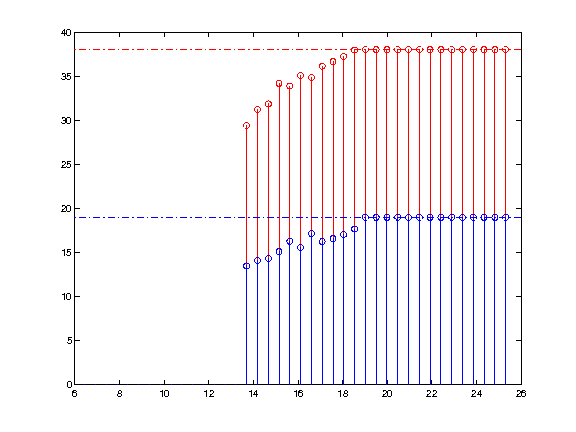
\includegraphics{test7}

The red bars are  the estimated means of $Y$ under the  estimated constrained optimal regimes vs. constraint value $\kappa$. The blue bars are  the estimated means of $Z$ under the estimated constrained optimal regime vs. constrain value $\kappa$. The red dash line is the estimated maximal of $Y$ without constraint, and the blue dash line is the estimated minimal of $Z$ without constraint. For the constrained problems, Matlab fmincon  solver is used with `Algorithm' option set to `interior-point' method, and `FinDiffRelStep' to 1e-2.  For unconstrained problems, Matlab fminunc solver is used,where `Algorithm' options is set to `quasi-newton', and `FinDiffRelStep' to 1e-2. MultiStart function is called for 5 random starts, where `StartPointsToRun' option is set to `all'.
% modeling conditional distributions
\end{comment}
% asymptotics for estimated indexing parm
\subsection{Asymptotic normality of $\wh{\bs{\theta}}_{\bs{\nu}}(\mu)$}
The asymptotic properties of $\wh{\bs{\theta}}_{\bs{\nu}}(\mu)$ here is similar to the corresponding part for one-stage problem in Chapter 1 (Section 1.1.6). 
\subsubsection{Limiting distribution of $\nabla\wh{V}_j(\bs{\theta})$}
Before we derive the limiting distribution of the estimator $\wh{\bs{\theta}}_{\kappa}(\mu)$, we need to examine, for any fixed value of $\bs{\theta}: \bs{\theta}_1^\itl\bs{\theta}_1 = 1$ and $\bs{\theta}_2^\itl\bs{\theta}_2 = 1$, the limiting distribution of $\nabla\wh{V}_j(\bs{\theta})$, where
\begin{flalign*}
\nabla\wh{V}_j(\bs{\theta}) = &\pard[\bs{\theta}] \int y \,d \wh{F}_{Y_j^*(\bs{\theta})}(y) \\
= &\pard[\bs{\theta}] \int y \,d \lt( \mean[n] \wh{F}_{Y^*(\bs{\theta})}(y | \bs{H}_{1,i} = \bs{h}_{1,i}) \rt)\\
= & \mean[n] \pard[\bs{\theta}] \int y \,d  \wh{F}_{Y_j^*(\bs{\theta})}(y | \bs{H}_{1,i} = \bs{h}_{1,i}),
\end{flalign*}
%\begin{gather}
%\begin{flalign*}
%\nabla_{\bs{\theta}}\wh{\mathbb{E}}\lt\{ \text{sgn}\lt(\bs{X}^{\intercal}\bs{\theta}\rt)\bs{X}_1^{\intercal}\bs{\beta}_{Y1}\rt\} =\nabla_{\bs{\theta}}\lt[\frac{1}{n}\sum_{i=1}^{n}\bs{X}_{i,1}^{\intercal}\bs{\beta}_{Y1}\lt\{ 1-2K\lt(-\frac{\bs{X}^{\intercal}_{i}\bs{\theta}}{h}\rt)\rt\} \rt]=\frac{1}{n}\sum_{i=1}^{n}\frac{2\bs{X}_{i,1}^{\intercal}\bs{\beta}_{Y1}}{h}k\lt(-\frac{\bs{X}_{i}^{\intercal}\bs{\theta}}{h}\rt)\bs{X}_{i}.
%\end{flalign*}
%\end{gather}
where $\wh{F}_{Y_j^*(\bs{\theta})}(\cdot)$ denote the estimator of $F_{Y^*_j(\bs{\theta})}(\cdot)$
\begin{lemma}
 Suppose the following conditions hold.
	\begin{enumerate}
		\item $\forall \bs{a} \in \mathbb{R}^p$,$\exists \delta > 0$ ,such that
		\begin{enumerate}
			\item $\mathbb{E}\lt|\bs{a}^\itl\pard[\bs{\theta}] \int y \,d  \wh{F}_{Y_j^*(\bs{\theta})}(y | \bs{H}_{1,i} = \bs{h}_{1,i})\rt|^{2+\delta} < \infty$
			\item $ \lt\{\bs{\bs{a}^{\intercal}}\text{Var}\lt[\pard[\bs{\theta}] \int y \,d  \wh{F}_{Y_j^*(\bs{\theta})}(y | \bs{H}_{1,i} = \bs{h}_{1,i})\rt]\bs{a} \rt\}^{1+\frac{\delta}{2}}< \infty$.
		\end{enumerate}
	\end{enumerate}
	Then, we have, for any fixed $\bs{\theta}$,
	\begin{gather}
	\begin{flalign*}
%	\sqrt{n}\lt(\nabla \wh{V}_j(\bs{\theta})  -\mathbb{E}\lt(\nabla \wh{V}_j(\bs{\theta})\rt)\rt)\overset{d}{\to}\mathcal{N}\lt(0,\text{Avar}\lt(\pard[\bs{\theta}] \int y \,d  \wh{F}_{Y_j^*(\bs{\theta})}(y | \bs{H}_{1,i} = \bs{h}_{1,i}) \rt) \rt)
	\end{flalign*}
	\end{gather}
\end{lemma}

The proof of this is similar to the proof of Lemma 1.1.3 and is shown in Appendix B.1.
%\subsection{Limiting distribution of $\nabla_{\bs{\theta}}\wh{\mathbb{E}}\lt\{ \text{sgn}\lt(\bs{X}^{\intercal}\bs{\theta}\rt)\bs{X}_1^{\intercal}\bs{\beta}_{Y1}\rt\} $}

%Comment: Goal is to prove the derivative above is asymptotically normal.
%Considering that it includes sample size $n$ in $h$, and it is multivariate.
%Try Lyapunov condition and cramer-wold theorem first.
%
%The sequences here are a triangular array, and are iid for each $n$.
%
%$k$ is the kernel of our choice, gaussian kernel.
Assume $\wh{F}_{Y_j^*(\bs{\theta})}(y | \bs{H}_{1,i} = \bs{h}_{1,i})$ is consistent, and the following corollary shows that the estimations do not effect the limiting distribution obtained above.
\begin{corollary}
	Suppose all the assumptions in Lemma 2.2.1  hold, and $\wh{F}_{Y_j^*(\bs{\theta})}(y | \bs{H}_{1,i} = \bs{h}_{1,i})$ is a consistent estimator of ${F}_{Y_j^*(\bs{\theta})}(y_j | \bs{H}_{1,i} = \bs{h}_{1,i})$. Then, we have
	\begin{gather}
	\begin{flalign*}
	\sqrt{n}\lt(\nabla \wh{V}_j(\bs{\theta}^*_{\bs{\nu}}(\mu))  - \nabla V_j(\bs{\theta}^*_{\bs{\nu}}(\mu))\rt)\overset{d}{\to}\mathcal{N}\lt(0,\text{Avar}\lt(\pard[\bs{\theta}] \int y_j \,d  F_{Y_j^*(\bs{\theta})}(y | \bs{H}_{1,i} = \bs{h}_{1,i})\bigg\rvert_{\bs{\theta} = \bs{\theta}^*_{\bs{\nu}}(\mu)} \rt)\rt)
	\end{flalign*}
	\end{gather}
\end{corollary}
See Appendix B.2 for proof.
\begin{comment}
\begin{proof}
	We write
	\begin{gather}
	\begin{flalign*}
	& \nabla \wh{V}_j(\bs{\theta})  - \nabla V_j^*(\bs{\theta}) \\
	= & \nabla \wh{V}_j(\bs{\theta})  - \mb{E}\lt(\nabla \wh{V}_j(\bs{\theta}) \rt) + \mb{E}\lt(\nabla \wh{V}_j(\bs{\theta}) \rt)- \nabla V_j^*(\bs{\theta}) ,
	\end{flalign*}
	\end{gather}
	where $ \mb{E}\lt(\nabla \wh{V}_j(\bs{\theta}) \rt)- \nabla V_j^*(\bs{\theta})=  \mb{E}\lt(\pard[\bs{\theta}]\int y_j \,d  \wh{F}_{Y_j^*(\bs{\theta})}(y | \bs{H}_{1,i} = \bs{h}_{1,i})\rt)  - \mb{E} \lt(\pard[\bs{\theta}]\int y_j \,d  F_{Y_j^*x(\bs{\theta})}(y_j| \bs{H}_{1,i} = \bs{h}_{1,i}\rt)$  $ = o_p(1)$, due to the consistency of $\wh{F}_{Y_j^*(\bs{\theta})}(y | \bs{H}_{1,i} = \bs{h}_{1,i})$ and dominated convergence theorem.\\
	
	In lemma 2.1.1, let $\bs{\theta} = \bs{\theta}^*_{\bs{\nu}}(\mu)$ and then
	\begin{gather}
	\begin{flalign*}
	\sqrt{n}\lt(\nabla \wh{V}_j(\bs{\theta}^*_{\bs{\nu}}(\mu))  - \nabla \mb{E}\lt( \wh{V}_j(\bs{\theta}^*_{\bs{\nu}}(\mu))\rt)\rt)\overset{d}{\to}\mathcal{N}\lt(0,AV\lt(\pard[\bs{\theta}] \int y_j \,d \wh{F}_{Y_j^*(\bs{\theta})}(y | \bs{H}_{1,i} = \bs{h}_{1,i})\bigg\rvert_{\bs{\theta} = \bs{\theta}^*_{\bs{\nu}}(\mu)} \rt)\rt).
	\end{flalign*}
	\end{gather}
	As $\wh{F}_{Y_j^*(\bs{\theta})}(y | \bs{H}_{1,i} = \bs{h}_{1,i})$ is consistent, we have
	\begin{gather*}
	\frac{AV\lt[\pard[\bs{\theta}] \int y \,d  \wh{F}_{Y_j^*(\bs{\theta})}(y | \bs{H}_{1,i} = \bs{h}_{1,i}) \rt]}{AV\lt[\pard[\bs{\theta}] \int y_j \,d  F_{Y^*(\bs{\theta})}(y | \bs{H}_{1,i} = \bs{h}_{1,i}) \rt]} \overset{p}{\to} 1.
	\end{gather*}
	Then, we have
	\begin{gather}
\begin{flalign*}
\sqrt{n}\lt(\nabla \wh{V}_j(\bs{\theta}^*_{\bs{\nu}}(\mu))  - \nabla \mb{E}\lt( \wh{V}_j(\bs{\theta}^*_{\bs{\nu}}(\mu))\rt)\rt)\overset{d}{\to}\mathcal{N}\lt(0,AV\lt(\pard[\bs{\theta}] \int y_j \,d \wh{F}_{Y_j^*(\bs{\theta})}(y | \bs{H}_{1,i} = \bs{h}_{1,i})\bigg\rvert_{\bs{\theta} = \bs{\theta}^*_{\bs{\nu}}(\mu)} \rt)\rt).
\end{flalign*}
\end{gather}
\end{proof}
\end{comment}

\subsubsection{Limiting distribution of $\wh{\bs{\theta}}_{\bs{\nu}}(\mu)$}
Now, we investigate the limiting distribution of $\wh{\bs{\theta}}_{\bs{\nu}}(\mu)$.
\begin{theorem}
	Suppose all the assumptions above hold. Then we have, as $n\to \infty$
	\begin{flalign*}
	\sqrt{n}(\wh{\bs{\theta}}_{\bs{\nu}}(\mu) - \bs{\theta}_{\bs{\nu}}(\mu)^*) \overset{d}{\to} \mathcal{N}\lt(\bs{0}, \bs{\Sigma}^* \rt),
	\end{flalign*}
	where $\bs{\Sigma}^* = \bs{D}^{*-1}\bs{C}^{*}\bs{D}^{*-1}$, \\
		$\bs{C}^* =\mathbb{E}\lt( \nabla v_1\lt(\bs{\theta}^*_{\bs{\nu}}(\mu)\rt)\nabla^{\itl} v_1\lt(\bs{\theta}^*_{\bs{\nu}}(\mu)\rt) \rt) - \mathbb{E}\lt(\nabla v_1\lt(\bs{\theta}^*_{\bs{\nu}}(\mu)\rt)\rt) \mathbb{E}\lt(\nabla^{\itl} v_1\lt(\bs{\theta}^*_{\bs{\nu}}(\mu)\rt)\rt)$,\\
	and $\bs{D}^*  =  \nabla^2 \phi^{BP}_{\mu}(\bs{\theta}^*_{\bs{\nu}}(\mu))$.
\end{theorem}
The proof is similar to the proof of Theorem 1.1.5, and is presented in Appendix B.3.
\begin{comment}
	\begin{flalign*}
	\bs{C}^* :=
	AV\lt[\pard[\bs{\theta}] \int y \,d F_{Y^*(\bs{\theta})}(y | \bs{H}_{1} = \bs{h}_{1}) \rt],
	\end{flalign*}
	and
	\begin{gather*}
	\begin{flalign*}
	\bs{D}^*:= &\nabla^2 \mb{E} Y^*(\bs{\theta}^*_{\bs{\nu}}(\mu)) - \mu \frac{\nabla^2 \mb{E} Z^*(\bs{\theta}^*_{\bs{\nu}}(\mu)) \lt[ \kappa - \mb{E} Z^*(\bs{\theta}^*_{\bs{\nu}}(\mu)) \rt] + \{ \nabla \mb{E} Z^*(\bs{\theta}^*_{\bs{\nu}}(\mu)) \}^2}{  \lt\{\kappa - \mb{E} Z^*(\bs{\theta}^*_{\bs{\nu}}(\mu)) \rt\}^2} \\
	= & \nabla^2 {S}^* (\bs{\theta}_{\bs{\nu}}(\mu)^*, \mu).
	\end{flalign*}
	\end{gather*}
\end{theorem}
\begin{proof}
	
	Taylor expansion, for each $\mu$
	$$\nabla\wh{S}(\bs{\theta}^*_{\bs{\nu}}(\mu),\mu) = \nabla\wh{S}(\wh{\bs{\theta}}_{\bs{\nu}}(\mu),\mu) - \nabla^2\wh{S}(\tilde{\bs{\theta}}_{\bs{\nu}}(\mu), \mu) (\wh{\bs{\theta}}_{\bs{\nu}}(\mu) - \bs{\theta}^*_{\bs{\nu}}(\mu) ),$$
	where $\tilde{\bs{\theta}}_{\bs{\nu}}(\mu)$ is a vector in between $\wh{\bs{\theta}}_{\bs{\nu}}(\mu)$ and $\bs{\theta}^*_{\bs{\nu}}(\mu)$.
	As $\wh{\bs{\theta}}_{\kappa}(\mu)$ is the maximizer of $\wh{S}(\bs{\theta}, \mu)$, it satisfies the first order conditions such that $\nabla\wh{S}(\wh{\bs{\theta}}_{\bs{\nu}}(\mu),\mu) = 0$. Then,
	\begin{flalign*}
	& \sqrt{n}\nabla\wh{S}(\bs{\theta}^*_{\bs{\nu}}(\mu),\mu) =  -\sqrt{n} \nabla^2\wh{S}(\tilde{\bs{\theta}}_{\bs{\nu}}(\mu),\mu ) (\wh{\bs{\theta}}_{\bs{\nu}}(\mu) - \bs{\theta}^*_{\bs{\nu}}(\mu) )\\
	& \nabla\wh{S}(\bs{\theta}^*_{\bs{\nu}}(\mu),\mu) = \nabla \wh{\mb{E}} Y_n(\bs{\theta}^*_{\bs{\nu}}(\mu)) - \mu \frac{\nabla \wh{\mb{E}} Z_n(\bs{\theta}^*_{\bs{\nu}}(\mu))}{  \kappa - \wh{\mb{E}} Z_n(\bs{\theta}^*_{\bs{\nu}}(\mu)) } + + \frac{2}{\mu}\,(\bs{\theta}_{\bs{\nu}}(\mu)^{*\intercal}\bs{\theta}^*_{\bs{\nu}}(\mu)-1)\bs{\theta}^*_{\bs{\nu}}(\mu),
	\txt{where }\bs{\theta}_{\bs{\nu}}(\mu)^{*\itl}\bs{\theta}^*_{\bs{\nu}}(\mu)-1 = 0.\\
	& \nabla^2\wh{S}(\bs{\theta}^*_{\bs{\nu}}(\mu), \mu) = \nabla^2 \wh{\mb{E}} Y_n(\bs{\theta}^*_{\bs{\nu}}(\mu)) - \mu \frac{\nabla^2 \wh{\mb{E}} Z_n(\bs{\theta}^*_{\bs{\nu}}(\mu)) \lt[ \kappa - \wh{\mb{E}} Z_n(\bs{\theta}^*_{\bs{\nu}}(\mu)) \rt] + \{ \nabla \wh{\mb{E}} Z_n(\bs{\theta}^*_{\bs{\nu}}(\mu)) \}^2}{  \lt\{\kappa - \wh{\mb{E}} Z_n(\bs{\theta}^*_{\bs{\nu}}(\mu)) \rt\}^2}
	\end{flalign*}
	Then, we have
	\begin{flalign*}
	\nabla\wh{S}(\bs{\theta}^*_{\bs{\nu}}(\mu),\mu) = \nabla \wh{\mb{E}} Y_n(\bs{\theta}^*_{\bs{\nu}}(\mu)) - \mu \frac{\nabla \wh{\mb{E}} Z_n(\bs{\theta}^*_{\bs{\nu}}(\mu))}{  \kappa - \wh{\mb{E}} Z_n(\bs{\theta}^*_{\bs{\nu}}(\mu)) },
	\end{flalign*}
	
	%As the left hand side is asymptotically normal with mean $\bs{0}$ and
	By Lemma 3, we have  the first term on the right hand side as
	\begin{gather}
	\begin{flalign*}
	\nabla \wh{V}_j(\bs{\theta})  \overset{d}{\to}\mathcal{N}\lt\{\nabla \mb{E}Y^*(\bs{\theta}),\frac{1}{n}AV\lt[\pard[\bs{\theta}] \int y \,d F_{Y^*(\bs{\theta})}(y | \bs{H}_{1} = \bs{h}_{1}) \rt]\rt\}
	\end{flalign*}
	\end{gather}
	For the second term on the right hand side, we also have that
	\begin{gather*}
	\mu \frac{\nabla \wh{\mb{E}} Z_n(\bs{\theta}^*_{\bs{\nu}}(\mu))}{  \kappa - \wh{\mb{E}} Z_n(\bs{\theta}^*_{\bs{\nu}}(\mu)) } \overset{p}{\to} \mu \frac{\nabla \mb{E} Z(\bs{\theta}^*_{\bs{\nu}}(\mu))}{  \kappa - \mb{E} Z(\bs{\theta}^*_{\bs{\nu}}(\mu)) },,
	\end{gather*}
	where we assume  both $\kappa - \wh{\mb{E}} Z_n(\bs{\theta}^*_{\bs{\nu}}(\mu)) > 0$ and $\kappa - \mb{E} Z(\bs{\theta}^*_{\bs{\nu}}(\mu)) > 0$ . This convergence in probabilty is due to the consistency of $\wh{F}_{Z_n(\bs{\theta})}(z | \bs{H}_1 = \bs{h}_1)$ and dominated convergence theorem. Together, by Sluskty's theorem and the stationarity of $\bs{\theta}^*_{\bs{\nu}}(\mu)$ of $S^*(\bs{\theta}, \mu)$, we have
	\begin{flalign*}
	\sqrt{n} \nabla\wh{S}( {\bs{\theta}}^*_{\bs{\nu}}(\mu), \mu) \overset{d}{\to} \mathcal{N}\lt(0, \bs{C}^*\rt),
	\end{flalign*}
	where
	\begin{flalign*}
	\bs{C}^* :=
	AV\lt[\pard[\bs{\theta}] \int y \,d F_{Y^*(\bs{\theta})}(y | \bs{H}_{1} = \bs{h}_{1}) \rt]
	\end{flalign*}
	
	We have that  $\nabla^2\wh{S}(\tilde{\bs{\theta}}_{\bs{\nu}}(\mu), \mu) = \nabla^2\wh{S}(\bs{\theta}^*_{\bs{\nu}}(\mu), \mu) + o_p(1)$,  as $\tilde{\bs{\theta}}_{\bs{\nu}}(\mu)$ is in between $\wh{\bs{\theta}}_{\bs{\nu}}(\mu)$ and $\bs{\theta}^*_{\bs{\nu}}(\mu)$ and $\wh{\bs{\theta}}_{\bs{\nu}}(\mu) - \bs{\theta}^*_{\bs{\nu}}(\mu) = o_p(1)$.
	Therefore, we have
	\begin{flalign*}
	\bs{D}^* \triangleq & p\underset{n \to \infty}{\lim}\nabla^2\wh{S}_{\kappa} (\bs{\theta}^*_{\kappa, \mu}, \mu) \\
	= & p\underset{n \to \infty}{\lim} \lt[\nabla^2 \wh{\mb{E}} Y_n(\bs{\theta}^*_{\bs{\nu}}(\mu)) - \mu \frac{\nabla^2 \wh{\mb{E}} Z_n(\bs{\theta}^*_{\bs{\nu}}(\mu)) \lt[ \kappa - \wh{\mb{E}} Z_n(\bs{\theta}^*_{\bs{\nu}}(\mu)) \rt] + \{ \nabla \wh{\mb{E}} Z_n(\bs{\theta}^*_{\bs{\nu}}(\mu)) \}^2}{  \lt\{\kappa - \wh{\mb{E}} Z_n(\bs{\theta}^*_{\bs{\nu}}(\mu)) \rt\}^2}\rt] \\
	= &\nabla^2 \mb{E} Y^*(\bs{\theta}^*_{\bs{\nu}}(\mu)) - \mu \frac{\nabla^2 \mb{E} Z^*(\bs{\theta}^*_{\bs{\nu}}(\mu)) \lt[ \kappa - \mb{E} Z^*(\bs{\theta}^*_{\bs{\nu}}(\mu)) \rt] + \{ \nabla \mb{E} Z^*(\bs{\theta}^*_{\bs{\nu}}(\mu)) \}^2}{  \lt\{\kappa - \mb{E} Z^*(\bs{\theta}^*_{\bs{\nu}}(\mu)) \rt\}^2} \\
	= & \nabla^2 {S}^* (\bs{\theta}_{\bs{\nu}}(\mu)^*, \mu).
	\end{flalign*}
\end{proof}
We can estimate $\bs{\Sigma}^*$ by plug in the corresponding estimators stated, and denote the estimator $\wh{\bs{\Sigma}}$, that is, $\wh{\bs{\Sigma}} = \wh{\bs{D}}^{-1}\wh{\bs{C}}\wh{\bs{D}}^{-1}$, where

\begin{flalign*}
\wh{\bs{C}} = & \wh{V}\lt\{\pard[\bs{\theta}] \int y \,d \wh{F}_{Y_n(\wh{\bs{\theta}}_{\bs{\nu}}(\mu))}(y | \bs{H}_{1} = \bs{h}_{1}) \rt\} \\
= & \wh{V} \lt[\nabla \wh{\mb{E}} \lt\{Y_n(\wh{\bs{\theta}}_{\bs{\nu}}(\mu)) \mid \bs{H}_1 =\bs{h_1}\rt\}\rt]
\end{flalign*}

and
\begin{gather*}
\begin{flalign*}
\wh{\bs{D}} =   \nabla^2\wh{S}(\wh{\bs{\theta}}_{\bs{\nu}}(\mu), \mu) = \nabla^2 \wh{\mb{E}} Y_n(\wh{\bs{\theta}}_{\bs{\nu}}(\mu)) - \mu \frac{\nabla^2 \wh{\mb{E}} Z_n(\wh{\bs{\theta}}_{\bs{\nu}}(\mu)) \lt[ \kappa - \wh{\mb{E}} Z_n(\wh{\bs{\theta}}_{\bs{\nu}}(\mu)) \rt] + \{ \nabla \wh{\mb{E}} Z_n(\wh{\bs{\theta}}_{\bs{\nu}}(\mu)) \}^2}{  \lt\{\kappa - \wh{\mb{E}} Z_n(\wh{\bs{\theta}}_{\bs{\nu}}(\mu)) \rt\}^2},
\end{flalign*}
\end{gather*}

As $\wh{\bs{C}}$ , $\wh{\bs{D}}$  and $\wh{\bs{\Sigma}}$ maybe have complicated forms, bootstrap based estimators can be used for practical dataset, and Monte Carlo estimators for simulated replicates.\\

\textbf{Confidence set of $\wh{\bs{\theta}}$}\\
As  Theorem 1 that
\begin{flalign*}
\bs{\Sigma}^{* -\sfrac{1}{2} }(\wh{\bs{\theta}}_{\bs{\nu}}(\mu) - \bs{\theta}_{\bs{\nu}}(\mu)^*) \overset{d}{\to} \mathcal{N}\lt(\bs{0}, \mathbf{I}/n \rt), \text{as } n \to \infty,
\end{flalign*}
we have
\begin{flalign*}
(\wh{\bs{\theta}}_{\bs{\nu}}(\mu) - \bs{\theta}_{\bs{\nu}}(\mu)^*)\bs{\Sigma}^{*-1}(\wh{\bs{\theta}}_{\bs{\nu}}(\mu) - \bs{\theta}_{\bs{\nu}}(\mu)^*) \overset{d}{\to} \chi^2_{p+1}/n^2, \text{as } n \to \infty.
\end{flalign*}
Thus, with a consistent estimator of $\wh{\bs{\Sigma}}$, the $(1 - \alpha) \times 100 \%$ confidence set is
\begin{flalign*}
\bs{\mathcal{C}}_{1-\alpha}\lt(\bs{\theta}^*_{\kappa, \mu}\rt)= \lt\{ \bs{\theta}_{\bs{\nu}}(\mu):
(\wh{\bs{\theta}}_{\bs{\nu}}(\mu) - \bs{\theta}_{\bs{\nu}}(\mu))\wh{\bs{\Sigma}}^{-1}(\wh{\bs{\theta}}_{\bs{\nu}}(\mu) - \bs{\theta}_{\bs{\nu}}(\mu)) \le \chi^2_{p+1}( 1-\alpha )/n^2 \rt\}, \txt{ as } n \to \infty,
\end{flalign*}
where $\chi^2_{p+1}( 1-\alpha )$ is the $1-\alpha$ quantiles of a $\chi_{p+1}^2$ random variable, and $p+1$ is the dimension of $\bs{\theta}$.\\

\textbf{Projection Confidence Interval of $\mb{E}Y^*(\bs{\theta}_{\kappa, \mu}^*)$}\\
For each $\bs{\theta}_{\kappa, \mu} \in \bs{\mathcal{C}}_{1-\alpha} \lt(\bs{\theta}^*_{\kappa, \mu}\rt)$, we estimate $\mb{E} Y^*(\bs{\theta}_{\kappa, \mu})$ by $\wh{\mb{E}} Y_n(\bs{\theta}_{\kappa, \mu}) = \mean[n] \int y \,d  \wh{F}_{Y_n(\bs{\theta}_{\kappa, \mu})}(y | \bs{H}_{1,i} = \bs{h}_{1,i})  $. Thus, assuming $\wh{F}_{Y_n(\bs{\theta}_{\bs{\nu}}(\mu))}(y | \bs{H}_{1,i} = \bs{h}_{1,i})$ is a consistent estimator of $F_{Y^*(\bs{\theta}_{\bs{\nu}}(\mu))}(y | \bs{H}_{1,i} = \bs{h}_{1,i})$ , $\wh{\mb{E}} Y_n(\bs{\theta}_{\kappa, \mu})$ has a limiting distribution as
$$\sqrt{n} \lt\{ \wh{\mb{E}}Y_n(\bs{\theta}_{\kappa, \mu})  - \mb{E} Y^*(\bs{\theta}_{\kappa, \mu}) \rt\} \sim  \mathcal{N}\lt[ 0 , AV\lt\{ \int y \,d  F_{Y^*(\bs{\theta}_{\bs{\nu}}(\mu))}(y | \bs{H}_{1,i} = \bs{h}_{1,i}) \rt\}\rt].$$
For each $\bs{\theta}_{\kappa, \mu} \in \bs{\mathcal{C}}_{1-\alpha} \lt(\bs{\theta}^*_{\kappa, \mu}\rt)$, we can construct a $(1 - \eta ) \times 100 \%$ confidence interval
\begin{flalign*}
&\bs{\mathcal{I}}_{1 -\eta} \lt\{ \mb{E}Y^*(\bs{\tau}_{\kappa, \mu})  \rt\} \\
= & \lt\{\wh{\mb{E}}Y_n(\bs{\tau}_{\kappa, \mu}) - Z_{1- \eta/2}  \wh{\sigma}_{Y^*(\bs{\tau}_{\bs{\nu}}(\mu))} ,  \wh{\mb{E}}Y_n(\bs{\tau}_{\kappa, \mu}) + Z_{1 - \eta/2} \wh{\sigma}_{Y^*(\bs{\tau}_{\bs{\nu}}(\mu))}  \rt\}
\end{flalign*}
where $\wh{\sigma}_{Y^*(\bs{\tau}_{\bs{\nu}}(\mu))}$ is the estimator for $AV\lt\{ \int y \,d  F_{Y^*(\bs{\tau}_{\bs{\nu}}(\mu))}(y | \bs{H}_{1,i} = \bs{h}_{1,i}) \rt\}$, which can also be calculated by bootstrap estimator  for practical dataset, or Monte Carlo estimator for simulated replicates.  $Z_{1- \eta/2}$ is the upper $1- \eta/2$ critical value for the standard normal distribution. Alternatively, we can also construct this confidence interval using standard methods such as percentile bootstrap. Then, we can construct the projection confidence set for $ \mb{E}Y^*\lt(\bs{\tau}_{\kappa, \mu}\rt)$ by taking the union of $\bs{\mathcal{I}}_{1 -\eta} \lt\{ \mb{E}Y^*\lt(\bs{\tau}_{\kappa, \mu}\rt)  \rt\}$ over all $\bs{\tau}_{\kappa, \mu} \in \bs{\mathcal{C}}_{1-\alpha} \lt(\bs{\tau}^*_{\kappa, \mu}\rt)$, i.e.,
$$
\bs{\mathcal{U}}_{1 - \alpha - \eta} \lt\{ \mb{E}Y^*(\bs{\tau}_{\kappa, \mu})  \rt\} = \bigcup_{\bs{\tau}_{\kappa, \mu} \in \bs{\mathcal{C}}_{1-\alpha} \lt(\bs{\tau}^*_{\kappa, \mu}\rt)} \bs{\mathcal{I}}_{1 -\eta} \lt\{ \mb{E}Y^*(\bs{\tau}_{\kappa, \mu})  \rt\}.
$$
\end{comment}
\section{Simulation}
\subsection{Simulation design}
We demonstrate our proposed method using the toy example presented by Linn et al~\cite{constrained}, where there are two competing outcomes $Y$ and $Z$. The goal is to maximize the mean of $Y$, subject to an upper bound on the mean of $Z$. $Y$ is coded so that the higher the value the better, such as the effectiveness of the treatment regimes. Meanwhile, $Z$ is coded the lower the better, such as the side-effect burden. The model for generating the patient trajectories $(X_1, A_1, X_2, A_2, Y, Z)$ are as follow:
\begin{flalign*}
&X_1 \sim \text{Normal}(1,1), \\
&\bs{H}_1 = (1, X_1)^{\itl}, \\
&A_1 \sim \text{Uniform}\left\{-1, 1\right\}, \\
&X_2 = \bs{H}_1^{\itl}\bs{\beta}_{1,0} + A_1\bs{H}_1^{\itl}\bs{\beta}_{1,1} + \epsilon, \\
&\epsilon \sim \text{Normal}(0,1), \\
&\bs{H}_2 = (1, X_2)^{\itl},\\
&A_2 \sim \text{Uniform}\left\{-1, 1\right\}, \\
&Y = \bs{H}_2^{\itl}\bs{\beta}_{2,0,Y} + A_2 \bs{H}_2^{\itl}\bs{\beta}_{2,1,Y}+\epsilon_Y \\
&Z = \bs{H}_2^{\itl}\bs{\beta}_{2,0,Z} + A_2 \bs{H}_2^{\itl}\bs{\beta}_{2,1,Z}+\epsilon_Z \\
&(\epsilon_Y, \epsilon_Z)^{\itl} \sim \text{Normal}(\bs{0}_2, \Sigma_{Y,Z}) 
\end{flalign*}
This model is a simple representation of the data from a two-stage randomized SMART. Variable $X_1$ represents the summary of patient status before the first treatment assignment $A_1$. Variable $X_2$ represents the summary of patient status before the second treatment assignment $A_2$. The parameters involved are set to the following,
\begin{flalign*}
&\bs{\beta}_{1,0} = (0.5, 0.75)^{\itl}\\
&\bs{\beta}_{1,1} = (0.25, 0.5)^{\itl}\\
&\bs{\gamma}_0 = (0.25, -0.05)^{\itl}\\
&\bs{\gamma}_1 = (0.1, -0.05)^{\itl}\\
&\bs{\beta}_{2,0,Y} = (30, 2)^{\itl}\\
&\bs{\beta}_{2,1,Y} = (5, -1.5)^{\itl}\\
&\bs{\beta}_{2,0,Z} = (15, 1)^{\itl}\\
&\bs{\beta}_{2,1,Z}=(3,-0.5)^{\itl}\\
&\Sigma_{Y,Z} = \begin{bmatrix}
1.0, &0.7 \\
0.7,& 1.0
\end{bmatrix}
\end{flalign*}
The class of regimes under consideration is restricted to linear decision rules at each stage. That is $\pi_1 = \text{sgn}(\bs{h}_1^{\itl}\bs{\theta}_1)$ and  $\pi_2 = \text{sgn}(\bs{h}_2^{\itl}\bs{\theta}_2)$, where $\bs{\theta}_1$ and $\bs{\theta}_2$ are the index parameters for the regimes. The true optimal regimes are denoted by $\pi^{*}_1 = \text{sgn}(\bs{h}_1^{\itl}\bs{\theta}^{*}_1)$ and  $\pi^{*}_2 = \text{sgn}(\bs{h}_2^{\itl}\bs{\theta}^{*}_2)$. The estimated optimal regimes are denoted by $\wh{\pi}_1 = \text{sgn}(\bs{h}_1^{\itl}\wh{\bs{\theta}}_1)$ and  $\wh{\pi}_2 = \text{sgn}(\bs{h}_2^{\itl}\wh{\bs{\theta}}_2)$. Here, the sgn function is defined as
 \begin{gather*}
\text{sgn}(x)=\begin{cases}
1 & \mbox{if }x\ge0,\\
-1 & \mbox{if }x<0.
\end{cases}
\end{gather*}
\subsection{Modeling and estimation}
\textbf{Modeling for and estimation of the distributions of potential outcomes}\\
The distribution of potential outcomes are unknown. The two major quantities under an arbitrary regime $\bs{\pi}$ involved, $\mb{E}Y^*(\bs{\pi})$ and $\mb{E}Z^*(\bs{\pi})$, need to be estimated from the observed data. Our strategy for estimating these two quantities is to model the marginal distribution of each potential outcome, and then draw random samples from the estimated marginal distributions to calculate their expectations numerically. To connect observed data with potential outcomes, three necessary causal inference assumptions $\textit{B1)-B3).}$ are assumed to hold. \\

%\begin{enumerate}
%	\item Consistency: $Y = Y^*(A_1, A_2)$.
%	\item Sequential ignorability: $A_t  \indep W^*  | \bs{H}_{t}$ for $t =1 ,2$.
%	\item Positivity: $\exists \epsilon > 0$ for which $\epsilon < \text{Pr}(A_t = a_t \mid \bs{H}_t) < 1 - \epsilon$ with probabilty one for all $a_t$, $t=1, 2$.
%\end{enumerate}
Following the G-computation formula~\cite{Gill2001}, we have, for any arbitrary regime $\bs{\pi} = (\pi_1, \pi_2) $, that
\begin{equation*}	
\resizebox{\textwidth}{!}{
$\text{Pr}\{ Y^*(\bs{\pi})) \le y\} = \mb{E}_{\bs{H}_1} \lt\{ \mb{E}_{\bs{H}_2}\lt[ \text{Pr}\lt\{Y \le y \mid \bs{H}_2 , A_2 = \pi_2(\bs{H}_2), \bs{H}_1 , A_1 = \pi_1(\bs{H}_1)\rt\}  \mid \bs{H}_1, A_1 = \pi_1(\bs{H}_1) \rt] \rt\}$
}
\end{equation*}

%\begin{equation*}	\
%\text{Pr}\{ Y^*(\bs{\pi}) > y\} =\mb{E} \left[ \underset{a_1}{\sum} \mathds{1}_{a_1 = d_1(\bs{H}_1)} \mb{E}\left\{ \underset{a_2}{\sum} \mathds{1}_{a_2 = d_2(\bs{H}_2)} \text{Pr} (Y > y \rvert \bs{X}_1 = \bs{x}_1, A_1 = a_1, \bs{X}_2 = \bs{x}_2, A_2=a_2)  \mid \bs{X}_1, A_1 = a_1\right\}\right],
%\end{equation*}
and similarly, 
\begin{equation*}
\resizebox{\textwidth}{!}{
$\text{Pr}\{ Z^*(\bs{\pi}) \le z\} =  \mb{E}_{\bs{H}_1} \lt\{ \mb{E}_{\bs{H}_2}\lt[  \text{Pr}\lt\{Z \le z \mid \bs{H}_2 , A_2 = \pi_2(\bs{H}_2), \bs{H}_1 , A_1 = \pi_1(\bs{H}_1)\rt\}  \mid \bs{H}_1, A_1 = \pi_1(\bs{H}_1) \rt] \rt\}$
}
\end{equation*}

%	\begin{gather*}
%	\begin{flalign*}
%	& \text{Pr}\{ Z^*(\bs{\pi}) > z\} =\\
%	& \mb{E} \left[ \underset{a_1}{\sum} \mathds{1}_{a_1 = d_1(\bs{H}_1)} \mb{E}\left\{ \underset{a_2}{\sum} \mathds{1}_{a_2 = d_2(\bs{H}_2)} \text{Pr} (Z > z \rvert \bs{X}_1 = \bs{x}_1, A_1 = a_1, \bs{X}_2 = \bs{x}_2, A_2=a_2) \rvert \bs{X}_1, A_1 = a_1\right\}\right].
%	\end{flalign*}
%	\end{gather*}

%\begin{flalign*}
%& \text{Pr}\{ Y^*(\bs{\pi}) > y\} =\\
%& \mb{E} \left[ \underset{a_1}{\sum} \mathds{1}_{a_1 = d_1(\bs{H}_1)} \mb{E}\left\{ \underset{a_2}{\sum} \mathds{1}_{a_2 = d_2(\bs{H}_2)} \text{Pr} (Y > y \rvert \bs{H}_2, A_2)  \mid \bs{H}_1, A_1 \right\}\right],
%\end{flalign*}

%\marginnote{\small{Review G-computation!}}[-1.5cm]
%\begin{flalign*}
%& \text{Pr}\{ Z^*(\bs{\pi}) > z\} =\\
%& \mb{E} \left[ \underset{a_1}{\sum} \mathds{1}_{a_1 = d_1(\bs{H}_1)} \mb{E}\left\{ \underset{a_2}{\sum} \mathds{1}_{a_2 = d_2(\bs{H}_2)} \text{Pr} (Z > z \rvert \bs{H}_2 , A_2 ) \mid \bs{H}_1 , A_1 \right\}\right].
%\end{flalign*}

Hence, we can estimate the probabilty function of the potential outcomes under a regime $\bs{\pi}$, $\text{Pr}\{ Y^*(\bs{\pi}) \le y\}$ and $\text{Pr}\{ Z^*(\bs{\pi}) \le z\}$  , using observed data by modeling and estimating the conditional distributions involved, and hence, $\mb{E}Z^*(\bs{\pi})$ and $\mb{E}Z^*(\bs{\pi})$.\\

Following the modeling tactic in ``Constrained estimation for competing outcomes" by Linn et al~\cite{constrained}. We assume the following model, 
\begin{flalign*}
& Y  = \mb{E}(Y \rvert \bs{H}_2, A_2)  + \varepsilon_Y,  \\
& \mb{E}(Y \rvert \bs{H}_2, A_2)  = m_Y(\bs{H}_2) + A_2 c_Y(\bs{H}_2), \\
& \text{where } \mb{E}(\varepsilon_Y) = 0, \text{Var}(\varepsilon_Y) = \sigma^2, \text{and } \varepsilon_Y \indep (\bs{H}_2, A_2).
\end{flalign*}

Define $F_{\varepsilon_Y}(\cdot)$ to be the distribution of $\varepsilon_Y$; $F_{\bs{H}_2 \rvert \bs{H}_1, A_1}(\cdot \mid \bs{h}_1, a_1)$ to be the conditional distribution of $\bs{H}_2$ given $\bs{H}_1 = \bs{h}_1$ and $A_1 = a_1$; $F_{\bs{H}_1}(\cdot)$ to be the distribution of $\bs{H}_1$. Again, we have $\bs{H}_1^\itl = (1, \bs{X}^\itl_1)$, $\pi_1(\bs{H}_1)$, $\bs{H}_2 = \{ \bs{H}^\itl_1, \pi_1(\bs{H}_1), \bs{X}^\itl_2\}^\itl$. \\	
%	Let $J^{d_1, d_2}(\bs{h}_1, \bs{h}_2, y) = F_{\varepsilon_Y}\{ y - m(\bs{h_2}^{d_1(\bs{h_1})}) - d_2(\bs{h}_2^{d_1(\bs{h}_1)})c_Y(\bs{h}_2^{d_1(\bs{h}_1)}) \}$, then
\begin{flalign*}
& \text{Pr}\lt\{ Y \le y \mid \bs{H}_2 =\bs{h}_2, \pi_2(\bs{H}_2) =\pi_2(\bs{h}_2) \rt\} \\
= & \text{Pr}\lt\{ m(\bs{H}_2 )+ \pi_2( \bs{H}_2)c_Y(\bs{H}_2) + \varepsilon_Y \le y \mid \bs{H}_2 =\bs{h}_2, \pi_2(\bs{H}_2) =\pi_2(\bs{h}_2)  \rt\} \\
= & \text{Pr}\lt\{ \varepsilon_Y \le y - m(\bs{H}_2) - \pi_2( \bs{H}_2)c_Y(\bs{H}_2) \mid \bs{H}_2 =\bs{h}_2, \pi_2(\bs{H}_2) =\pi_2(\bs{h}_2) \rt\}\\
=&  F_{\varepsilon_Y}\lt\{ y - m(\bs{h}_2) - \pi_2(\bs{h}_2)c_Y(\bs{h}_2) \rt\}\\
= &  F_{\varepsilon_Y}\lt[ y - m(\bs{h}_2) - \tsgn\lt\{r_2(\bs{h}_2; \bs{\theta}_2)\rt\}c_Y(\bs{h}_2) \rt]
\end{flalign*}
Hence, we have
\begin{flalign*}
& \text{Pr}\lt\{ Y^*({\bs{\pi}}) \le y  \rt\} \\  
= &  \iint \text{Pr}\lt\{ Y \le y \mid  \bs{H}_2=\bs{h}_2, A_2 = \pi_2(\bs{h}_2) \rt\} \,d F_{\bs{H}_2 \mid \bs{H}_1, A_1}\lt\{ \bs{h}_2 \rvert \pi_1(\bs{\bs{h}_1}), \bs{h}_1 \rt\} \,d F_{\bs{H}_1}(\bs{h}_1)\\
= &  \iint  F_{\varepsilon_Y}\lt\{ y - m(\bs{h}_2) - \pi_2(\bs{h}_2)c_Y(\bs{h}_2) \rt\} \,d F_{\bs{H}_2 \mid  \bs{H}_1, A_1}\lt\{ \bs{h}_2 \mid \bs{h}_1 , \pi_1(\bs{h}_1)\rt\} \,d F_{\bs{H}_1}(\bs{h}_1)\\
% = & \iint  F_{\varepsilon_Y}\lt\{ y - m_Y(\bs{h}_2) - \pi_2(\bs{h}_2)c_Y(\bs{h}_2) \rt\} \,d G_{Y}\lt\{ m_Y, c_Y \rvert \bs{h}_1 , d_1(\bs{h}_1)\rt\} \,d F_{\bs{H}_1}(\bs{h}_1) \\
= &  \iint  F_{\varepsilon_Y}\lt[ y - m(\bs{h}_2) - \tsgn\lt\{r_2(\bs{h}_2; \bs{\theta}_2)\rt\}c_Y(\bs{h}_2) \rt] \,d G_{Y}\lt\{ m_Y, c_Y, r_2 \rvert \bs{h}_1 , \pi_1(\bs{h}_1)\rt\} \,d F_{\bs{H}_1}(\bs{h}_1) \\
= &  \iint  F_{\varepsilon_Y}\lt[ y - m(\bs{h}_2) - \tsgn(r_2)c_Y(\bs{h}_2) \rt] \,d G_{Y}\lt\{ m_Y, c_Y, r_2 \rvert \bs{h}_1 , \pi_1(\bs{h}_1)\rt\} \,d F_{\bs{H}_1}(\bs{h}_1) 
\end{flalign*}
where $G_{Y}\lt\{ m_Y , c_Y, r_2\mid \bs{h}_1, a_1 \rt\}$ is the joint conditional distribution of $m_Y\lt(\bs{H}_2\rt)$, $c_Y\lt(\bs{H}_2\rt)$ and $r_2(\bs{H}_2; \bs{\theta}_2)$ given $\bs{H}_1 = \bs{h}_1$ and $A_1 = a_1$. The second equality is due to \\ 
$\int z(x, y) \,d F_{X | Y}(x | y) = \mb{E}(z | y) = \int z\,d F_{Z | Y}(z | y).$\\

Same applies to $Z$:
\begin{flalign*}
& Z  = \mb{E}(Z \rvert \bs{H}_2, A_2)  + \epsilon, \\
& \text{where } \mb{E}(\epsilon) = 0, \text{Var}(\epsilon) = \sigma^2, \text{and } \epsilon \indep (\bs{H}_2, A_2) \\
& \mb{E}(Z \rvert \bs{H}_2, A_2)  = m_Z(\bs{H}_2) + A_2 c_Z(\bs{H}_2)
\end{flalign*}
\begin{flalign*}
& \text{Pr}\lt\{ Z^*(\bs{\pi}) \le z  \rt\} \\  
= &  \iint \text{Pr}\lt\{ Z \le z \mid  \bs{H}_2=\bs{h}_2, \pi_2(\bs{H}_2)= \pi_2(\bs{h}_2) \rt\} \,d F_{\bs{H}_2 \mid \bs{H}_1, A_1}\lt\{ \bs{h}_2 \rvert d_1(\bs{\bs{h}_1}), \bs{h}_1 \rt\} \,d F_{\bs{H}_1}(\bs{h}_1)\\
= &  \iint  F_{\varepsilon_Z}\lt\{ z - m(\bs{h}_2) - \pi_2(\bs{h}_2)c_Z(\bs{h}_2) \rt\} \,d F_{\bs{H}_2 \mid  \bs{H}_1, A_1}\lt\{ \bs{h}_2 \mid \bs{h}_1 , \pi_1(\bs{h}_1)\rt\} \,d F_{\bs{H}_1}(\bs{h}_1)\\
% = & \iint  F_{\varepsilon_Z}\lt\{ z - m_Z(\bs{h}_2) - \pi_2(\bs{h}_2)c_Z(\bs{h}_2) \rt\} \,d G_{Z}\lt\{ m_Z, c_Z \rvert \bs{h}_1 , d_1(\bs{h}_1)\rt\} \,d F_{\bs{H}_1}(\bs{h}_1) \\
= &  \iint  F_{\varepsilon_Z}\lt[ z - m(\bs{h}_2) - \tsgn\lt\{r_2(\bs{h}_2; \bs{\theta}_2)\rt\}c_Z(\bs{h}_2) \rt] \,d G_{Z}\lt\{ m_Z, c_Z, r_2 \rvert \bs{h}_1 , \pi_1(\bs{h}_1)\rt\} \,d F_{\bs{H}_1}(\bs{h}_1) \\
= &  \iint  F_{\varepsilon_Z}\lt[ z - m(\bs{h}_2) - \tsgn(r_2)c_Z(\bs{h}_2) \rt] \,d G_{Z}\lt\{ m_Z, c_Z, r_2 \rvert \bs{h}_1 , \pi_1(\bs{h}_1)\rt\} \,d F_{\bs{H}_1}(\bs{h}_1) 
\end{flalign*}

where $G_{Z}\lt\{ m_Z, c_Z, r_2 \mid \bs{h}_1, a_1 \rt\}$ is the joint conditional distribution of $m_Z\lt(\bs{H}_2\rt)$, $c_Z\lt(\bs{H}_2\rt)$ and $r_2(\bs{H}_2; \bs{\theta}_2)$ given $\bs{H}_1 = \bs{h}_1$ and $A_1 = a_1$. \\

%\subsubsection*{Estimating $G^{\pi_2}_{Y,Z}( \cdot,	\cdot,\cdot,\cdot,\cdot \mid X_1 = x_1, A_1 = a_1)$}
We model the joint distribution of $\lt\{ m_Y(\bs{H}_2), c_Y(\bs{H}_2), m_Z(\bs{H}_2), c_Z(\bs{H}_2) \rt\}$ by modeling the joint distribution of the standardized residuals obtained from the mean and variance modeling of each component for given $\bs{H}_1$ and $A_1$ 
\begin{flalign*}
e^m_Y = \frac{m_Y(\bs{H}_2) - \mu_Y^m(\bs{H}_1, A_1)}{\sigma_Y^m(\bs{H}_1, A_1)} \\
e^c_Y = \frac{c_Y(\bs{H}_2) - \mu_Y^c(\bs{H}_1, A_1)}{\sigma_Y^c(\bs{H}_1, A_1)} \\
e^m_Z = \frac{m_Z(\bs{H}_2) - \mu_Z^m(\bs{H}_1, A_1)}{\sigma_Z^m(\bs{H}_1, A_1)} \\
e^c_Z = \frac{c_Z(\bs{H}_2) - \mu_Z^c(\bs{H}_1, A_1)}{\sigma_Z^c(\bs{H}_1, A_1)} \\
e_{f_2} = \frac{f_2(\bs{H}_2) - \mu_{f_2}(\bs{H}_1, A_1)}{\sigma_{f_2}(\bs{H}_1, A_1)}
\end{flalign*}
The mean functions are defined as 
\begin{flalign*}
\mu_Y^m(\bs{H}_1, A_1) = \mb{E}\{ m_Y(\bs{H}_2) \mid \bs{H}_1, A_1 \} \\
\mu_Y^c(\bs{H}_1, A_1) = \mb{E}\{ c_Y(\bs{H}_2) \mid \bs{H}_1, A_1 \} \\
\mu_Z^m(\bs{H}_1, A_1) = \mb{E}\{ m_Z(\bs{H}_2) \mid \bs{H}_1, A_1 \} \\
\mu_Z^c(\bs{H}_1, A_1) = \mb{E}\{ c_Z(\bs{H}_2) \mid \bs{H}_1, A_1 \} \\
\mu_{f_2}(\bs{H}_1, A_1) = \mb{E}\{ f_2(\bs{H}_2) \mid \bs{H}_1, A_1 \}
\end{flalign*}
and the standard deviation functions are defined as
\begin{flalign*}
&\sigma_Y^m(\bs{H}_1, A_1) = \mb{E} \big[\{ m_Y(\bs{H}_2) - \mu_Y^m(\bs{H}_1, A_1) \}^2\mid \bs{H}_1, A_1 \big]^{1/2} \\
&\sigma_Y^c(\bs{H}_1, A_1) = \mb{E} \big[ \{ c_Y(\bs{H}_2) - \mu_Y^c(\bs{H}_1, A_1) \}^2\mid \bs{H}_1, A_1 \big]^{1/2}\\
&\sigma_Z^m(\bs{H}_1, A_1) = \mb{E} \big[ \{ m_Z(\bs{H}_2) - \mu_Z^m(\bs{H}_1, A_1) \}^2\mid \bs{H}_1, A_1 \big]^{1/2}\\
&\sigma_Z^c(\bs{H}_1, A_1) = \mb{E} \big[ \{ c_Z(\bs{H}_2) - \mu_Z^c(\bs{H}_1, A_1) \}^2\mid \bs{H}_1, A_1 \big]^{1/2}\\
&\sigma_{f_2}(\bs{H}_1, A_1) = \mb{E} \big[ \{ f_2(\bs{H}_2) - \mu_{f_2}(\bs{H}_1, A_1) \}^2\mid \bs{H}_1, A_1 \big]^{1/2}
\end{flalign*}
Therefore, we model the joint distribution of the standardized residuals $(e^m_Y, e^c_Y, e^m_Z, e^c_Z, e_{f_2})$ to obtain an estimator of $G_{Y,Z}^{\pi}(\cdot, \cdot, \cdot, \cdot, \cdot \mid x_1, a_1 )$.\\

%\subsubsection*{Parametric models for $m_Y(\bs{H}_2), c_Y(\bs{H}_2), m_Z(\bs{H}_2), c_Z(\bs{H}_2)\text{ and }f_2(\bs{H}_2)$ }
Due to the cost of clinical data, sample sizes are usually small. We consider parametric models for $m_Y(\bs{H}_2), c_Y(\bs{H}_2), m_Z(\bs{H}_2), c_Z(\bs{H}_2)\text{ and }f_2(\bs{H}_2)$. Here, we model $m_{Y}(\bs{H}_2)=\bs{H}_1^{\itl}\bs{\alpha}_1+A_1\bs{H}^{\itl}_1\bs{\alpha}_2+\varepsilon,$ where $\varepsilon$ is a mean-zero error term. Then, $\mu_Y^m(\bs{H}_1, A_1) = \bs{H}_1^{\itl}\bs{\alpha}_1+A_1\bs{H}^{\itl}_1\bs{\alpha}_2.$\\

To estimate, we fit the corresponding least squares regressions, and estimate the residuals empirically. For more details, see reference~\cite{constrained}.
%Details of estimation and modeling follows ``Estimation of dynamic treatment regimes for complex outcomes: Balancing benefits and risks" by Linn et al.\\
\begin{comment}
\textbf{Estimation of the barrier trajectory} \\
Once we have the estimators of $\mb{E}Y^*(\bs{\theta})$ and $\mb{E}Z^*(\bs{\theta})$, denoted by $\wh{\mb{E}}Y_n(\bs{\theta})$ and $\wh{\mb{E}}Z_n(\bs{\theta})$, we plug  those estimators into Problem (2), and get Problem (3) as
\begin{equation}
\underset{\bs{\theta}}{\max }\,\, \wh{\mb{E}} Y_n(\bs{\theta}) + \mu \txt{log} \lt\{ \kappa - \wh{\mb{E}} Z_n(\bs{\theta}) \rt\} - \frac{1}{2\mu} \lt\{ (\bs{\theta}_1^\itl \bs{\theta}_1 -1 )^2 + (\bs{\theta}_2^\itl \bs{\theta}_2 -1 )^2 \rt\}
\end{equation}
Denote a solution to Problem (3) by $\wh{\bs{\theta}}_{\kappa}(\mu) = (\wh{\bs{\theta}}^\itl_{\kappa,\mu,1} , \wh{\bs{\theta}}_{\kappa,\mu,2}^\itl )^\itl$, and $\widehat{S}(\bs{\theta}, \mu) = \wh{\mb{E}} Y_n(\bs{\theta}) + \mu \, \txt{log} \lt\{ \kappa - \wh{\mb{E}}Z_n(\bs{\theta}) \rt\} - \frac{1}{2\mu} \lt\{ (\bs{\theta}_1^\itl \bs{\theta}_1 -1 )^2 + (\bs{\theta}_2^\itl \bs{\theta}_2 -1 )^2 \rt\}.$ The following figure is an replication of the simulation result in the ``Estimation of dynamic treatment regimes for complex outcomes" chapter.\\


%\begin{overpic}[width=0.90\textwidth]{test7}
%	\put (0, 57) {$\wh{\mb{E} }Y_n(\wh{\bs{\theta}}_{\kappa,\mu})$}
%	\put (0, 27) {$\wh{\mb{E} }Z_n(\wh{\bs{\theta}}_{\kappa,\mu})$}
%	\put (50, 2.5) {$\kappa$}
%\end{overpic}
%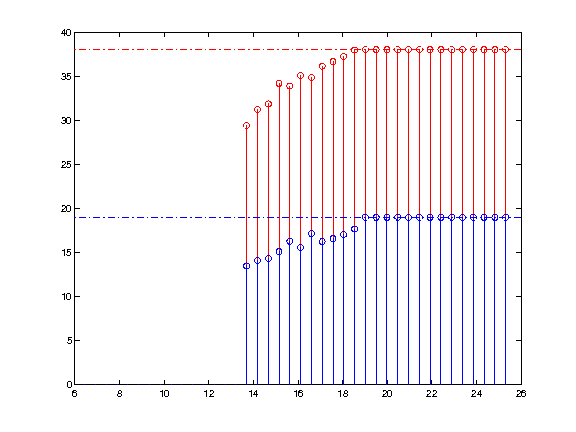
\includegraphics{test7}

The red bars are  the estimated means of $Y$ under the  estimated constrained optimal regimes vs. constraint value $\kappa$. The blue bars are  the estimated means of $Z$ under the estimated constrained optimal regime vs. constrain value $\kappa$. The red dash line is the estimated maximal of $Y$ without constraint, and the blue dash line is the estimated minimal of $Z$ without constraint. For the constrained problems, Matlab fmincon  solver is used with `Algorithm' option set to `interior-point' method, and `FinDiffRelStep' to 1e-2.  For unconstrained problems, Matlab fminunc solver is used,where `Algorithm' options is set to `quasi-newton', and `FinDiffRelStep' to 1e-2. MultiStart function is called for 5 random starts, where `StartPointsToRun' option is set to `all'.  
\end{comment}
\subsection{Summary of simulation results}
We summarize the simulation results here. Figure 2. below shows the estimated optimal regime values and their standard deviation. Figure 2.1 is the efficient frontier plot. The red dashed line represents $\wh{V}_1$ under estimated constrained optimal regime, and the blue dash-dotted line represents $\wh{V}_2$ under that regime. The plot represents the best possible value of the primary potential outcome for its level of risk, which is the value of the secondary potential outcome. In the plot, the value of the primary outcome increases as the constraint bound gets looser. Meanwhile the value of the secondary outcome keep up with the constraint, until the constraint is not active. Once the constraint gets larger than the maximum value of the secondary potential outcome, the constrained problem becomes an unconstrained problem. \\
\begin{center}
\begin{table}[!htbp]
\caption{Simulation results}
	\centering
{\tt
	\begin{tabular}{rrrrr}\hline 
$\nu$  & $\wh{V}_1(\wh{\bs{\theta}}_{\nu})$ & $std(\wh{V}_1)$ & $\wh{V}_2(\wh{\bs{\theta}}_{\nu})$ & $std(\wh{V}_2)$ \\ \hline 
   12.86 &    27.48 &     0.46  &    12.86 &      0.23  \\ 
   13.45 &    28.90 &     0.42  &    13.37 &      0.15  \\ 
   14.03 &    30.38 &     0.64  &    13.89 &      0.17  \\ 
   14.62 &    31.85 &     0.83  &    14.46 &      0.16  \\ 
   15.21 &    33.53 &     0.64  &    15.05 &      0.13  \\ 
   15.79 &    34.47 &     0.70  &    15.64 &      0.14  \\ 
   16.38 &    35.47 &     0.94  &    16.15 &      0.29  \\ 
   16.97 &    36.33 &     0.93  &    16.68 &      0.40  \\ 
   17.55 &    37.08 &     0.87  &    17.31 &      0.41  \\ 
   18.14 &    37.62 &     0.51  &    17.89 &      0.31  \\ 
   18.72 &    37.79 &     0.72  &    18.32 &      0.44  \\ 
   19.31 &    38.03 &     0.17  &    18.91 &      0.10  \\ 
   19.90 &    38.03 &     0.17  &    18.91 &      0.10  \\ 
   20.48 &    38.03 &     0.17  &    18.91 &      0.10  \\ 
   21.07 &    38.03 &     0.17  &    18.91 &      0.10  \\ 
   21.66 &    38.03 &     0.17  &    18.91 &      0.10  \\ 
   22.24 &    38.03 &     0.17  &    18.91 &      0.10  \\ 
   22.83 &    38.03 &     0.17  &    18.91 &      0.10  \\ 
   23.41 &    38.03 &     0.17  &    18.91 &      0.10  \\ 
   24.00 &    38.03 &     0.17  &    18.91 &      0.10  \\ \hline 
\end{tabular}

}
\justify
Here, $\nu$ denotes the values of the constraint; $\wh{V}_1(\wh{\bs{\theta}}_{\nu})$ denotes the values of estimated regimes in terms of primary outcome of interest; $std(\wh{V}_1)$ denotes the standard deviation of the estimated regime values in terms of primary outcome of interest; $\wh{V}_2(\wh{\bs{\theta}}_{\nu})$ denotes the values of estimated regimes in terms of secondary outcome of interest; $std(\wh{V}_2)$ denotes the standard deviation of the estimated regime values in terms of secondary outcome of interest.
\end{table}
\end{center}
\begin{figure}[H]
	\centering
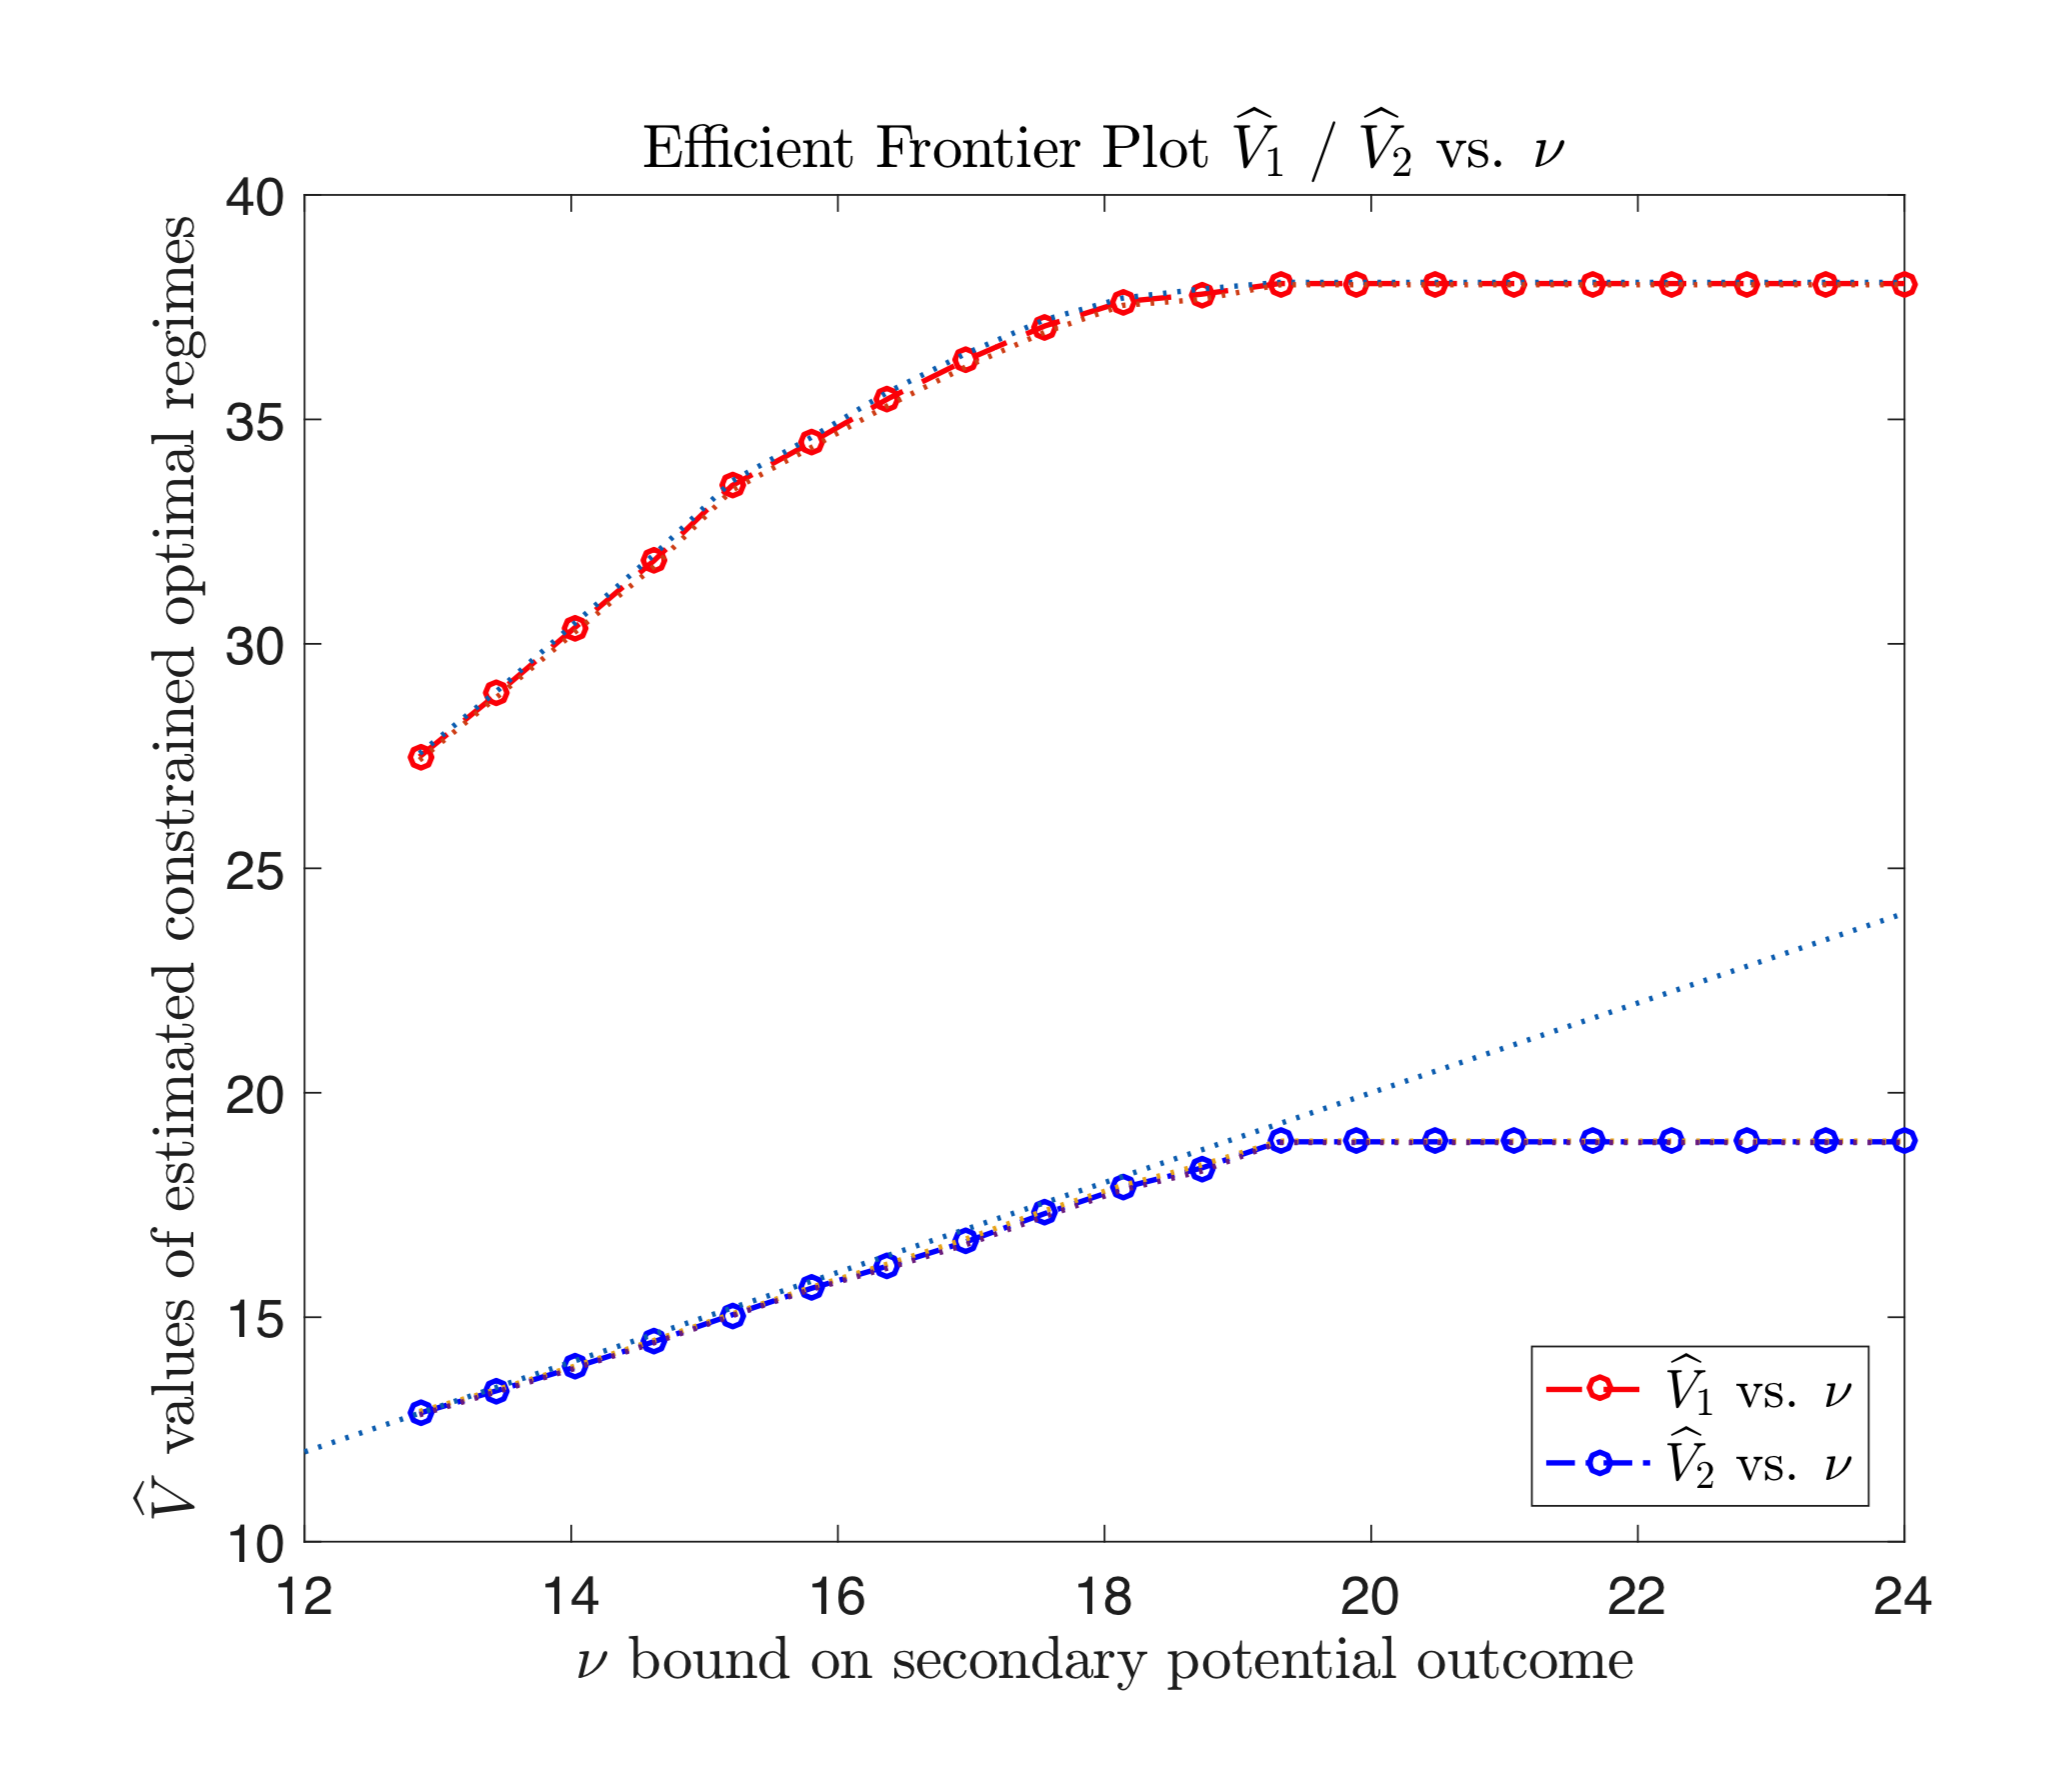
\includegraphics[width=0.9\linewidth]{./figs/efficient_plot.png}
\caption{Efficient frontier for estimated constrained optimal regimes (multi-stage)}
\justify
X-axis is for the values for the constraints $\nu$; Y-axis is for the values of estimated regimes. Red dashed line is for the values in terms of the primary outcome of interest. Blue dashed line is for the values in terms of the secondary outcome of interest.
\end{figure}


\section{Conclusion}
Focusing on optimizing a single scalar outcome may be an oversimplification of the goals of practical clinical decision making. In this chapter, a new method is proposed to handle multiple competing outcomes in the multi-stage setting. Estimating an optimal treatment regime with competing outcomes is cast as a constrained optimization problem. We maximize the primary outcome of interest, subject to the constraints on the secondary outcomes of interest. Our estimator of a constrained optimal treatment regime has the properties of consistency and asymptotic normality under mild regularity conditions. The efficient frontier plots provide an intuitive visualization for clinicians to examine the trade-off between two competing outcomes. 

\bibliography{ShupingR-thesis}{}
\bibliographystyle{plain}

\begin{appendices}
\section{Proof of Lemma 2.1.1}
\begin{lemma}
 Suppose the following conditions hold.
	\begin{enumerate}
		\item $\forall \bs{a} \in \mathbb{R}^p$,$\exists \delta > 0$ ,such that
		\begin{enumerate}
			\item $\mathbb{E}\lt|\bs{a}^\itl\pard[\bs{\theta}] \int y \,d  \wh{F}_{Y_j^*(\bs{\theta})}(y | \bs{H}_{1,i} = \bs{h}_{1,i})\rt|^{2+\delta} < \infty$
			\item $ \lt\{\bs{\bs{a}^{\intercal}}V\lt[\pard[\bs{\theta}] \int y \,d  \wh{F}_{Y_j^*(\bs{\theta})}(y | \bs{H}_{1,i} = \bs{h}_{1,i})\rt]\bs{a} \rt\}^{1+\frac{\delta}{2}}< \infty$.
		\end{enumerate}
	\end{enumerate}
	Then, we have, for any fixed $\bs{\theta}$,
	\begin{gather}
	\begin{flalign*}
	\sqrt{n}\lt(\nabla \wh{V}_j(\bs{\theta})  -\mathbb{E}\lt(\nabla \wh{V}_j(\bs{\theta})\rt)\rt)\overset{d}{\to}\mathcal{N}\lt(0,AV\lt(\pard[\bs{\theta}] \int y \,d  \wh{F}_{Y_j^*(\bs{\theta})}(y | \bs{H}_{1,i} = \bs{h}_{1,i}) \rt)\rt)
	\end{flalign*}
	\end{gather}
\end{lemma}

The proof of this is similar to the proof of Lemma 1.1.3 and is shown in APPENDIX.
%\subsection{Limiting distribution of $\nabla_{\bs{\theta}}\wh{\mathbb{E}}\lt\{ \text{sgn}\lt(\bs{X}^{\intercal}\bs{\theta}\rt)\bs{X}_1^{\intercal}\bs{\beta}_{Y1}\rt\} $}

%Comment: Goal is to prove the derivative above is asymptotically normal.
%Considering that it includes sample size $n$ in $h$, and it is multivariate.
%Try Lyapunov condition and cramer-wold theorem first.
%
%The sequences here are a triangular array, and are iid for each $n$.
%
%$k$ is the kernel of our choice, gaussian kernel.

\begin{proof}
	For any  $\bs{a} \in \mathbb{R}^p$, we let $W_{ni} = \bs{a}^\itl \pard[\bs{\theta}]\int y \,d  \wh{F}_{Y_j^*(\bs{\theta})}(y | \bs{H}_{1,i} = \bs{h}_{1,i})$. For each value of $n$, $w_{n1},w_{n2},\cdots,w_{nn}$ are i.i.d, and functions of the sample size $n$. This is because that $\bs{X}_{i}$ are assumed to be i.i.d., and $h$ is a function of sample
	size $n$. Then, we have
	\begin{gather*}
	\mu_{n}:=\mathbb{E}W_{ni}=\mathbb{E}\lt(\bs{a}^\itl \pard[\bs{\theta}]\int y \,d  \wh{F}_{Y_j^*(\bs{\theta})}(y | \bs{H}_{1,i} = \bs{h}_{1,i})\rt),
	\end{gather*}
	and
	\begin{gather*}
	\sigma_{n}^{2}:=V(W_{ni})=\bs{a}^\itl V\lt(\pard[\bs{\theta}]\int y \,d  \wh{F}_{Y_j^*(\bs{\theta})}(y | \bs{H}_{1,i} = \bs{h}_{1,i}) \rt)\bs{a}
	\end{gather*}
	
	%?????????????????????????????????????????????????????????? \\
	%??? Delta method and Taylor expansion for approximation ??? \\
	%?????????????????????????????????????????????????????????? \\
	We let $G_{ni}=W_{ni}-\mu_{\ensuremath{n}}$, and $T_{n}=\sum_{i=1}^{n}G_{ni}$. Also, we let $s_{n}^{2}=V(T_{n})=\sum_{i=1}^{n}V(G_{ni})=\sum_{i=1}^{n}\sigma_{n}^{2}=n\sigma_{n}^{2}$, where the second equality is because of independence, and the last equality is due to identicalness. Therefore, $\sfrac{T_{n}}{s_{n}}$ has mean 0, and variance 1.  If we can show $G_{ni}$ satisfying the Lyapunov condition, then
	we have
	
	$$\frac{T_{n}}{s_{n}}\overset{d}{\to}\mathcal{N}(0,1),\text{ as } n \to \infty$$,
	
	
	
	Now, we check the Lyapunov condition, that is, ~\cite{Lindsay1995,Hunter2014}
	\begin{gather*}
	\exists\delta>0, \text{ such that } \frac{1}{s_{n}^{2+\delta}}\sum_{i=1}^{n}\mathbb{E}\mid G_{n,i}\mid^{2+\delta}\to0, \text{ as } n\to0.
	\end{gather*}
	We define, for any $\bs{a}$,
	\begin{gather*}
	C_1 \triangleq \mathbb{E}\lt|G_{ni}\rt|^{2+\delta}=\mathbb{E}\lt|W_{ni}-\mu_{\ensuremath{n}}\rt|^{2+\delta}=\mathbb{E}\lt|\bs{a}^\itl \pard[\bs{\theta}]\int y \,d  \wh{F}_{Y_j^*(\bs{\theta})}(y | \bs{H}_{1,i} = \bs{h}_{1,i})-\mu_{n}\rt|^{2+\delta},
	\end{gather*}
	and
	\begin{gather*}
	C_2 \triangleq s_{n}^{2+\delta}=n^{1+\frac{\delta}{2}}\sigma_{n}^{2+\delta}=n^{1+\frac{\delta}{2}}\lt\{ \bs{a}^\itl  V \lt[ \pard[\bs{\theta}]\int y \,d  \wh{F}_{Y_j^*(\bs{\theta})}(y | \bs{H}_{1,i} = \bs{h}_{1,i}) \rt] \bs{a} \rt\} ^{1+\frac{\delta}{2}}.
	\end{gather*}
	Then, we have
	\begin{flalign*}
	&\frac{1}{s_{n}^{2+\delta}}\sum_{i=1}^{n}\mathbb{E}\mid G_{n,i}\mid^{2+\delta}\\
	=&\frac{\mathbb{E}\lt|\bs{a}^\itl \pard[\bs{\theta}]\int y \,d  \wh{F}_{Y_j^*(\bs{\theta})}(y | \bs{H}_{1,i} = \bs{h}_{1,i})-\mu_{n}\rt|^{2+\delta}}{n^{\frac{\delta}{2}}\lt\{ \bs{a}^{\intercal}V\lt[\pard[\bs{\theta}]\int y \,d  \wh{F}_{Y_j^*(\bs{\theta})}\lt(y | \bs{H}_{1,i} = \bs{h}_{1,i}\rt) \rt]\bs{a}\rt\} ^{1+\frac{\delta}{2}}} \\
	=&\frac{C_{1}}{n^{\frac{\delta}{2}}C_{2}}.
	\end{flalign*}
	
	As long as $\delta>0$, for finite $C_1$ and finite $C_2$, we have $\sfrac{C_{1}}{n^{\frac{\delta}{2}}C_{2}}\to0$,
	as $n\to\infty$. This means that the Lyapunov condition is satisfied, if $\mathbb{E}\lt|G_{ni}\rt|^{2+\delta}$ and $s_{n}^{2+\delta}$ are finite. Then,  by Lyapunov Central Limit Theorem, we have
	\begin{gather*}
	\frac{T_{n}}{s_{n}}\overset{d}{\to}\mathcal{N}(0,1).
	\end{gather*}
	
	As this hold for any arbitary non-random vector $\bs{a}\in \mathbb{R}^p$, we have, by Cramer-Wold Theorem, that
	\begin{gather*}
	\sqrt{n}\lt[\mean[n] \pard[\bs{\theta}]\int y \,d  \wh{F}_{Y_j^*(\bs{\theta})}(y | \bs{H}_{1,i} = \bs{h}_{1,i}) -\mathbb{E}\lt\{ \pard[\bs{\theta}]\int y \,d  \wh{F}_{Y_j^*(\bs{\theta})}(y | \bs{H}_{1,i} = \bs{h}_{1,i})\rt\}\rt]\overset{d}{\to}\mathcal{N}\lt(0,V\lt[\pard[\bs{\theta}]\int y \,d  \wh{F}_{Y_j^*(\bs{\theta})}(y | \bs{H}_{1,i} = \bs{h}_{1,i})\rt]\rt),
	\end{gather*}
	as $n \to \infty$. We denote $\bs{L}_{ni}= \pard[\bs{\theta}]\int y \,d  \wh{F}_{Y_j^*(\bs{\theta})}(y | \bs{H}_{1,i} = \bs{h}_{1,i})$,
	then this is written as
	\begin{gather*}
	\sqrt{n}\lt[\frac{1}{n}\sum_{i=1}^{n}\bs{L}_{ni}-\mathbb{E}\bs{L}_{n1}\rt]\overset{d}{\to}\mathcal{N}\lt(0,V\lt[\bs{L}_{n1}\rt]\rt).
	\end{gather*}
	Then, we have
	\begin{gather*}
	\frac{1/n\sum_{i=1}^{n}\bs{L}_{ni}-\mathbb{E}\bs{L}_{n1}}{[V(\bs{L}_{n1})/n]^{1/2}}\frac{[V(\bs{L}_{n1})/n]^{1/2}}{\lt[AV(\bs{L}_{n1})/n\rt]^{1/2}}\overset{d}{\to}\mathcal{N}(0,1).
	\end{gather*}
	As  $n \to \infty$,
	\begin{gather*}
	\frac{V(\bs{L}_{n1})^{1/2}}{AV(\bs{L}_{n1})^{1/2}}\to1,
	\end{gather*}
	then we have
	\begin{gather*}
	\frac{1/n\sum_{i=1}^{n}\bs{L}_{ni}-\mathbb{E}\bs{L}_{n1}}{[AV(\bs{L}_{n1})/n]^{1/2}}\overset{d}{\to}\mathcal{N}(0,1),
	\end{gather*}
	i.e.,
	\begin{gather*}
	\sqrt{n}\lt[1/n\sum_{i=1}^{n}\bs{L}_{ni}-\mathbb{E}\bs{L}_{n1}\rt]\overset{d}{\to}N\lt(0,AV(\bs{L}_{n1})\rt).
	\end{gather*}
	As $\frac{1}{n}\sum_{i=1}^{n}\bs{L}_{ni} =\mean[n] \pard[\bs{\theta}]\int y \,d  \wh{F}_{Y_j^*(\bs{\theta})}(y | \bs{H}_{1,i} = \bs{h}_{1,i}) = \nabla \wh{V}_j(\bs{\theta})$, we have
	\begin{gather}
	\begin{flalign*}
	\sqrt{n}\lt[\nabla \wh{V}_j(\bs{\theta})  -\mathbb{E}\lt\{\nabla \wh{V}_j(\bs{\theta})\rt\}\rt]\overset{d}{\to}\mathcal{N}\lt(0,AV\lt[\pard[\bs{\theta}] \int y \,d  \wh{F}_{Y_j^*(\bs{\theta})}(y | \bs{H}_{1,i} = \bs{h}_{1,i}) \rt]\rt)
	\end{flalign*}
	\end{gather}
\end{proof}
\section{Proof of Corollary 2.1.2}
\begin{corollary}
	Suppose all the assumptions in Lemma 3  hold, and $\wh{F}_{Y_j^*(\bs{\theta})}(y | \bs{H}_{1,i} = \bs{h}_{1,i})$ is a consistent estimator of ${F}_{Y_j^*(\bs{\theta})}(y_j | \bs{H}_{1,i} = \bs{h}_{1,i})$. Then, we have
	\begin{gather}
	\begin{flalign*}
	\sqrt{n}\lt(\nabla \wh{V}_j(\bs{\theta}^*_{\bs{\nu}}(\mu))  - \nabla V_j(\bs{\theta}^*_{\bs{\nu}}(\mu))\rt)\overset{d}{\to}\mathcal{N}\lt(0,AV\lt(\pard[\bs{\theta}] \int y_j \,d  F_{Y_j^*(\bs{\theta})}(y | \bs{H}_{1,i} = \bs{h}_{1,i})\bigg\rvert_{\bs{\theta} = \bs{\theta}^*_{\bs{\nu}}(\mu)} \rt)\rt)
	\end{flalign*}
	\end{gather}
\end{corollary}
\begin{proof}
	We write
	\begin{gather}
	\begin{flalign*}
	& \nabla \wh{V}_j(\bs{\theta})  - \nabla V_j^*(\bs{\theta}) \\
	= & \nabla \wh{V}_j(\bs{\theta})  - \mb{E}\lt(\nabla \wh{V}_j(\bs{\theta}) \rt) + \mb{E}\lt(\nabla \wh{V}_j(\bs{\theta}) \rt)- \nabla V_j^*(\bs{\theta}) ,
	\end{flalign*}
	\end{gather}
	where $ \mb{E}\lt(\nabla \wh{V}_j(\bs{\theta}) \rt)- \nabla V_j^*(\bs{\theta})=  \mb{E}\lt(\pard[\bs{\theta}]\int y_j \,d  \wh{F}_{Y_j^*(\bs{\theta})}(y | \bs{H}_{1,i} = \bs{h}_{1,i})\rt)  - $\\$\mb{E} \lt(\pard[\bs{\theta}]\int y_j \,d  F_{Y_j^*x(\bs{\theta})}(y_j| \bs{H}_{1,i} = \bs{h}_{1,i}\rt)$  $ = o_p(1)$, due to the consistency of $\wh{F}_{Y_j^*(\bs{\theta})}(y | \bs{H}_{1,i} = \bs{h}_{1,i})$ and dominated convergence theorem.\\
	
	In lemma 2.1.1, let $\bs{\theta} = \bs{\theta}^*_{\bs{\nu}}(\mu)$ and then
	\begin{gather}
	\begin{flalign*}
	\sqrt{n}\lt(\nabla \wh{V}_j(\bs{\theta}^*_{\bs{\nu}}(\mu))  - \nabla \mb{E}\lt( \wh{V}_j(\bs{\theta}^*_{\bs{\nu}}(\mu))\rt)\rt)\overset{d}{\to}\mathcal{N}\lt(0,AV\lt(\pard[\bs{\theta}] \int y_j \,d \wh{F}_{Y_j^*(\bs{\theta})}(y | \bs{H}_{1,i} = \bs{h}_{1,i})\bigg\rvert_{\bs{\theta} = \bs{\theta}^*_{\bs{\nu}}(\mu)} \rt)\rt).
	\end{flalign*}
	\end{gather}
	As $\wh{F}_{Y_j^*(\bs{\theta})}(y | \bs{H}_{1,i} = \bs{h}_{1,i})$ is consistent, we have
	\begin{gather*}
	\frac{AV\lt[\pard[\bs{\theta}] \int y \,d  \wh{F}_{Y_j^*(\bs{\theta})}(y | \bs{H}_{1,i} = \bs{h}_{1,i}) \rt]}{AV\lt[\pard[\bs{\theta}] \int y_j \,d  F_{Y^*(\bs{\theta})}(y | \bs{H}_{1,i} = \bs{h}_{1,i}) \rt]} \overset{p}{\to} 1.
	\end{gather*}
	Then, we have
	\begin{gather}
	\begin{flalign*}
	\sqrt{n}\lt(\nabla \wh{V}_j(\bs{\theta}^*_{\bs{\nu}}(\mu))  - \nabla V_j\lt(\bs{\theta}^*_{\bs{\nu}}(\mu)\rt)\rt)\overset{d}{\to}\mathcal{N}\lt(0,AV\lt(\pard[\bs{\theta}] \int y_j \,d F_{Y_j^*(\bs{\theta})}(y | \bs{H}_{1,i} = \bs{h}_{1,i})\bigg\rvert_{\bs{\theta} = \bs{\theta}^*_{\bs{\nu}}(\mu)} \rt)\rt).
	\end{flalign*}
	\end{gather}
\end{proof}

\section{Proof of Theorem 2.1.3}
\begin{theorem}
	Suppose all the assumptions above hold. Then we have, as $n\to \infty$
	\begin{flalign*}
	\sqrt{n}\lt(\wh{\bs{\theta}}_{\bs{\nu}}(\mu) - \bs{\theta}_{\bs{\nu}}(\mu)^*\rt) \overset{d}{\to} \mathcal{N}\lt(\bs{0}, \bs{\Sigma}^* \rt),
	\end{flalign*}
	where $\bs{\Sigma}^* = \bs{D}^{*-1}\bs{C}^{*}\bs{D}^{*-1}$, 	\\$\bs{C}^* =\mathbb{E}\lt( \nabla v_1\lt(\bs{\theta}^*_{\bs{\nu}}(\mu)\rt)\nabla^{\itl} v_1\lt(\bs{\theta}^*_{\bs{\nu}}(\mu)\rt) \rt) - \mathbb{E}\lt(\nabla v_1\lt(\bs{\theta}^*_{\bs{\nu}}(\mu)\rt)\rt) \mathbb{E}\lt(\nabla^{\itl} v_1\lt(\bs{\theta}^*_{\bs{\nu}}(\mu)\rt)\rt)$,\\
	and $\bs{D}^*  =  \nabla^2 \phi^{BP}_{\mu}(\bs{\theta}^*_{\bs{\nu}}(\mu))$.
\end{theorem}
\begin{proof} For notation simplicity in this proof, let $\phi\lt(\bs{\theta}\rt) = \phi^{PB}_{\mu}\lt(\bs{\theta}\rt)$ and $\wh{\phi}(\bs{\theta}) = \wh{\phi}^{PB}_{\mu}\lt(\bs{\theta}\rt)$ for this proof. Also, let $\bs{\theta}^* = \bs{\theta}^*_{\nu}(\mu)$ and $\wh{\bs{\theta}} = \wh{\bs{\theta}}_{\nu}(\mu)$ here.
	Recall $ \wh{\phi}(\bs{\theta}) = \wh{v}_1(\bs{\theta}) - \mu \sum_{j=2}^J \ln \wh{v}_j(\bs{\theta}) + \frac{1}{2\mu}\sum_{t=1}^{T}(\bs{\theta}^{\itl}_t\bs{\theta}_t - 1)^2$.  As  $\bs{\theta}_t^{\itl}\bs{\theta}_t-1=0$ is always satisfied as a constraint, the gradient is $\nabla\wh{\phi}\lt(\bs{\theta}\rt) = \,\,\nabla\wh{v}_1(\bs{\theta}) - \mu \sum_{j=2}^J \sfrac{\nabla\wh{v}_j\lt( \bs{\theta}\rt)}{\wh{v}_j\lt( \bs{\theta}\rt)}$. Taylor expansion of $\nabla\wh{\phi}\lt(\bs{\theta}^*\rt)$ at $\bs{\theta} = \widehat{\bs{\theta}}$ shows that
	\begin{flalign*}
	\nabla\wh{\phi}\lt(\bs{\theta}^*\rt) =  \nabla\wh{\phi}(\wh{\bs{\theta}})- \nabla^2\wh{\phi}(\tilde{\bs{\theta}}) (\widehat{\bs{\theta}} - \bs{\theta}^{*}) + o_p(1),
	\end{flalign*}
	where $\tilde{\bs{\theta}}$ is between $\wh{\bs{\theta}}$ and $\bs{\theta}^*$. As $\widehat{\bs{\theta}}$ is the maximizer of $\widehat{\phi}\lt(\bs{\theta}\rt)$, it satisfies the first order condition that $\nabla \wh{\phi}(\widehat{\bs{\theta}}) = 0$. Therefore, 
	\begin{flalign}
	\sqrt{n}\nabla\wh{\phi}\lt(\bs{\theta}^*\rt) =   - \sqrt{n} \nabla^2\wh{\phi}( \tilde{\bs{\theta}}) (\widehat{\bs{\theta}} - \bs{\theta}^{*}),
	\end{flalign}
	where $\nabla\wh{\phi}\lt(\bs{\theta}\rt) = \,\,\nabla\wh{v}_1(\bs{\theta}) - \mu \sum_{j=2}^J \sfrac{\nabla\wh{v}_j\lt( \bs{\theta}\rt)}{\wh{v}_j\lt( \bs{\theta}\rt)}$.
	Recall $v_1\lt(\bs{\theta}\rt)=- V_1\lt(\bs{\theta}\rt)$ and  $v_j\lt(\bs{\theta}\rt) = V_j\lt(\bs{\theta}\rt) - \nu_j$, for $j = 2, \cdots, J$.  Due to Corollary 2.1.2, together with (A.4) and (A.5),
	\begin{flalign}
	\sqrt{n}\bigg(\nabla\wh{v}_1(\bs{\theta}^*) - \nabla v_1(\bs{\theta}^*)\bigg)\overset{d}{\to}N\lt( 0, \bs{C}^*\rt),
	\end{flalign}
		where $\bs{C}^*=AV\bigg(\nabla v_1(\bs{\theta}^*)\bigg) =\mathbb{E}\lt\{  \nabla v_1(\bs{\theta}^*)\nabla^{\itl} v_1(\bs{\theta}^*) \rt\} - \mathbb{E}\nabla v_1(\bs{\theta}^*) \mathbb{E}\nabla^{\itl} v_1(\bs{\theta}^*)$\\
		$ = AV\lt(\pard[\bs{\theta}]\int y \,d  F_{Y_j^*(\bs{\theta})}(y | \bs{H}_{1,i} )\rt)$. That is,
%	\begin{gather*}
%	\begin{flalign*}
%	\bs{C}^* \triangleq =&AV\bigg(\nabla v_1(\bs{\theta}^*)\bigg)=
%	AV\lt[\frac{2\bs{X}_1^{\itl}\bs{\beta}^*_{1}}{h}k\lt(-\frac{\bs{X}^{\itl}\bs{\theta}^*}{h}\rt)\bs{X} \rt] = p\lim_{n \to \infty} V\lt[\frac{2\bs{X}_1^{\itl}\bs{\beta}^*_{1}}{h}k\lt(-\frac{\bs{X}^{\itl}\bs{\theta}^*}{h}\rt)\bs{X} \rt] \\
%	= & p\underset{n \to \infty}\lim \lt[ \mathbb{E} \lt\{ \frac{4\bs{\beta}^{*\itl}_{1}\bs{X}_1\bs{X}_1^{\itl}\bs{\beta}^*_{1}}{h^2}k^2\lt(-\frac{\bs{X}^{\itl}\bs{\theta}^*}{h}\rt)\bs{X}\bs{X}^{\itl}\rt\} -  \mathbb{E}\lt\{\frac{2\bs{X}_1^{\itl}\bs{\beta}^*_{1}}{h}k\lt(-\frac{\bs{X}^{\itl}\bs{\theta}^*}{h}\rt)\bs{X}\rt\} \mathbb{E}\lt\{\frac{2\bs{X}_1^{\itl}\bs{\beta}^*_{1}}{h}k\lt(-\frac{\bs{X}^{\itl}\bs{\theta}^*}{h}\rt)\bs{X}\rt\}^{\itl} \rt] \\
%	= & \mathbb{E}\lt\{  4\big(\bs{X}_1^{\itl}\bs{\beta}^*_{1}\delta\lt(\bs{X}^{\itl}\bs{\theta}^*\rt)\big)^2\bs{X}\bs{X}^{\itl} \rt\} - \mathbb{E}\lt\{2\bs{X}_1^{\itl}\bs{\beta}^*_{1}\delta\lt(\bs{X}^{\itl}\bs{\theta}^*\rt)\bs{X}\rt\} \mathbb{E}\lt\{2\bs{X}_1^{\itl}\bs{\beta}^*_{1}\delta\lt(\bs{X}^{\itl}\bs{\theta}^*\rt)\bs{X}\rt\}^{\itl}\\
%	=& \mathbb{E}\lt\{  \nabla v_1(\bs{\theta}^*)\nabla^{\itl} v_1(\bs{\theta}^*) \rt\} - \mathbb{E}\lt\{\nabla v_1(\bs{\theta}^*)\rt\} \mathbb{E}\lt\{\nabla^{\itl} v_1(\bs{\theta}^*)\rt\}.
%	\end{flalign*}
%	\end{gather*}
	Then, due to (B.1) and (B.2), we have
	\begin{flalign}
	\sum_{j=2}^J \frac{\nabla\wh{v}_j\lt( \bs{\theta}\rt)}{\wh{v}_j\lt( \bs{\theta}\rt)} -  \sum_{i=2}^{J}\frac{\nabla v_j(\bs{\theta})}{v_j(\bs{\theta})} = o_p(1).
	\end{flalign}
	Note $v_j(\bs{\theta}) > 0$, for $j =2, \cdots, J$, is implied by the log barrier operator. Put (B.2) and (B.3) together by Slutsky's theorem, we have
	\begin{flalign*}
	\sqrt{n}\lt\{\lt(\nabla\wh{v}_1(\bs{\theta}^*) - \mu \sum_{j=2}^J \frac{\nabla\wh{v}_j\lt( \bs{\theta}^*\rt)}{\wh{v}_j( \bs{\theta}^*)}\rt) - \lt(\nabla v_1(\bs{\theta}^*) - \mu \sum_{i=2}^{J}\frac{\nabla v_j(\bs{\theta}^*)}{v_j(\bs{\theta}^*)}\rt)\rt\}\overset{d}{\to}N\lt(0, \bs{C}^*\rt),
	\end{flalign*} 
	Due to the stationarity of $\bs{\theta}^*$, $\nabla \phi(\bs{\theta}^*)=\nabla v_1(\bs{\theta}^*) - \mu \sum_{i=2}^{J}\sfrac{\nabla v_j(\bs{\theta}^*)}{v_j(\bs{\theta}^*)} =0$. Together with Sluskty's theorem, we have 
	\begin{flalign*}
	\sqrt{n} \nabla\wh{\phi}( \bs{\theta}^*) \overset{d}{\to} N\lt(0, \bs{C}^*\rt),
	\end{flalign*}
	where 
	$\bs{C}^* =\mathbb{E}\lt\{  \nabla v_1(\bs{\theta}^*)\nabla^{\itl} v_1(\bs{\theta}^*) \rt\} - \mathbb{E}\lt\{\nabla v_1(\bs{\theta}^*)\rt\} \mathbb{E}\lt\{\nabla^{\itl} v_1(\bs{\theta}^*)\rt\}.$ \\
	
	As $	\sqrt{n}\nabla\wh{\phi}\lt(\bs{\theta}^*\rt) =  - \sqrt{n} \nabla^2\wh{\phi}( \tilde{\bs{\theta}}) (\widehat{\bs{\theta}} - \bs{\theta}^{*})$ stated in (A.7),we have
	\begin{flalign}
	\sqrt{n} \nabla^2\wh{\phi}( \tilde{\bs{\theta}}) (\widehat{\bs{\theta}} - \bs{\theta}^{*}) \overset{d}{\to} N(0, \bs{C}^*)
	\end{flalign} 	
	The Hessian is $\nabla^2\wh{\phi}\lt(\bs{\theta}\rt) = \,\,\nabla^2\wh{v}_1(\bs{\theta}) - \mu \sum_{j=2}^J \sfrac{\big(\nabla^2\wh{v}_j\lt( \bs{\theta}\rt)\wh{v}_j\lt( \bs{\theta}\rt)- \lt(\nabla\wh{v}_j\lt( \bs{\theta}\rt)\rt)^2\big)}{\wh{v}^2_j\lt( \bs{\theta}\rt)}$. Based on (A.4) and (A.5), we have
	\begin{gather}
	\begin{flalign}
	\bs{D}^* \triangleq & p\lim_{n \to \infty}\nabla^2\wh{\phi}\lt(\bs{\theta}^*\rt) =  \nabla^2 \phi(\bs{\theta}^*)
	=\nabla^2{v}_1(\bs{\theta}^*) - \mu \sum_{j=2}^J \frac{\nabla^2{v}_j\lt( \bs{\theta}^*\rt)v_j\lt( \bs{\theta}^*\rt)- \lt\{\nabla v_j\lt( \bs{\theta}^*\rt)\rt\}^2}{v^2_j\lt( \bs{\theta}^*\rt)}.
	\end{flalign}
	\end{gather}
	
	As $\tilde{\bs{\theta}}$ is a vector in-between $\bs{\theta}^*$ and $\wh{\bs{\theta}}$, we have $\nabla^2\wh{\phi}(\tilde{\bs{\theta}}) = \nabla^2\wh{\phi}(\bs{\theta}^*) + o_p(1)$. Therefore, based on (A.10) and (A.11), we have 
	\begin{flalign*}
	\sqrt{n}\lt(\widehat{\bs{\theta}} - \bs{\theta}^*\rt) \overset{d}{\to} N\lt(\bs{0}, \bs{\Sigma}^* \rt),
	\end{flalign*}
	where $\bs{\Sigma}^* = \bs{D}^{*-1}\bs{C}^{*}\bs{D}^{*-1}$, 
	$\bs{C}^* =\mathbb{E}\lt\{  \nabla v_1(\bs{\theta}^*)\nabla^{\itl} v_1(\bs{\theta}^*) \rt\} - \mathbb{E}\nabla v_1(\bs{\theta}^*) \mathbb{E}\nabla^{\itl} v_1(\bs{\theta}^*)$ and $\bs{D}^*  =  \nabla^2 \phi(\bs{\theta}^*)$.
\end{proof}
\end{appendices}
\end{document}